\documentclass{article}

\usepackage[T1]{fontenc}
\usepackage[utf8]{inputenc}
\usepackage{graphicx}
\usepackage[font=small,labelfont=bf]{caption}
\usepackage{booktabs, siunitx}
\usepackage{tikz}
\usepackage{tikz-qtree}
\usepackage{pifont}
\usepackage[margin=0.90in]{geometry}
\usepackage{etoolbox,titling}
\usepackage{enumitem}
\usepackage{fancyhdr}
\usepackage{soulutf8}
\usepackage{epigraph}
\usepackage{amssymb}
\usepackage{amsmath}

\pagestyle{fancy}
\fancyhf{}
\rhead{Chiara Solito}
\lhead{Dispense di Laboratorio di Bioinformatica}
\rfoot{Pagina \thepage}
\lfoot{Bioinformatica - A.A. 2021/22}
\usetikzlibrary{trees}
\tikzstyle{every node}=[draw=black,thick,anchor=west]
\newcommand{\angstrom}{\mbox{\normalfont\AA}}

\begin{document}
\newcommand\tab[1][0.3cm]{\hspace*{#1}}


\begin{titlepage}
    \begin{center}
        \vspace*{1cm}
            
        \Huge
        \textbf{Laboratorio di Bioinformatica}
            
        \vspace{0.5cm}
        \LARGE
        Dispense del corso - Modulo 1
            
        \vspace{1.5cm}
            
        \textbf{Chiara Solito}

        \vspace{0.8cm}

            
        \Large
        Corso di Laurea in Bioinformatica\\
        Università degli studi di Verona\\
        A.A. 2021/22
            
    \end{center}
\end{titlepage}
La presente è una dispensa riguardante il corso di \textbf{Laboratorio di Bioinformatica} del CdS in Bioinformatica (Università degli Studi di Verona). Per la stesura di questa dispensa si è fatta fede al materiale didattico fornito direttamente dal professore nell'Anno Accademico 2021/2022. Eventuali variazioni al programma successive al suddetto anno non saranno quindi incluse.\\
Insieme a questo documento in formato PDF viene fornito anche il codice \LaTeX  con cui è stato generato.
\tableofcontents
\thispagestyle{empty}
\newpage
\thispagestyle{empty}
\section{Il corso}
Il corso si propone di presentare allo studente le basi teoriche e applicative di algoritmi e programmi utilizzati nella ricerca e nell'analisi dei dati contenuti nelle principali banche dati biologiche di uso cor-rente. Il corso si compone di due moduli di seguito specificati.\\
Modulo 1: In questo modulo verranno appresi gli strumenti volti all'utilizzo dell'informazione in prote-omica, genomica, biochimica, biologia molecolare e strutturale. Si fornisce inoltre un'introduzione all'analisi e la visualizzazione di dati strutturali relativi a macromolecole biologiche e loro complessi e la creazione di semplici modelli dinamici e statici di reti biomolecolari, che avvicinerà lo studente all'emergente disciplina della systems biology.\\
Modulo 2: In questo modulo lo studente acquisirà conoscenza pratica degli strumenti bioinformatici per l'analisi, l'interpretazione e la predizione di dati biologici in proteomica, genomica, biochimica, biologia molecolare e strutturale. 
In particolare, gli studenti avranno la possibilità di applicare stru-menti della boinformatica allo stato dell'arte a specifici problemi biologici.
\begin{titlepage}
    \begin{center}
        \vspace*{1cm}
        \LARGE
        \textbf{Lezione 1: Introduzione}
            
        \vspace{1.5cm}
        
        \large
        Ripasso delle basi e introduzione dei concetti fondamentali

        \vspace{0.8cm}

    \end{center}
\end{titlepage}
\setcounter{page}{5}
\section{Cos'è la bioinformatica?}
La bioinformatica è (oggi) una disciplina scientifica dedicata alla risoluzione di problemi biologici a livello
molecolare con metodi informatici. Descrive fenomeni biologici in modo numerico/statistico.
\\
La bioinformatica principalmente:
    \begin{itemize}
        \item Fornisce modelli per l'interpretazione di dati provenienti da esperimenti di biologia molecolare e biochimica al fine di identificare tendenze e leggi numeriche
        \item genera nuovi strumenti matematici per l'analisi di sequenze di DNA, RNA e proteine (frequenza di sequenze rilevanti, loro evoluzione e funzione).
        \item organizza le conoscenze acquisite in basi di dati al fine di rendere tali dati accessibili a tutti, ottimizzando gli algoritmi di ricerca dei dati
    \end{itemize}
Condivide alcuni argomenti con:
    \begin{itemize} 
        \item \textbf{Systems biology}
            \subitem{-} Rappresenta i processi biologici come sistemi per comprenderne le funzioni e i principi in modo olistico per mezzo di modelli matematici
        \item \textbf{Computational biology}
            \subitem{-} Integra i risultati sperimentali con quelli derivanti da esperimenti in silico, ottenuti quindi per mezzo di metodi informatici a partire da dati biologici.
    \end{itemize}
\subsection{Il flusso dell'informazione biologica}
Ad ogni livello di organizzazione (da interazioni fra biomolecole fino a cellule, organismi,
popolazioni) l'elemento unificante è l'EVOLUZIONE, unico vero fondamento
teorico della disciplina.\\
\begin{itemize}
    \item EVOLUZIONE: adattamento progressivo attraverso
    variabilita' genetica casuale e selezione naturale (Darwin,
    1859)
    \item Ad ogni livello biologico, il fenotipo (insieme di tratti e
    caratteri somatici) è codificato dal genotipo (il patrimonio
    genetico)
    \item Genotipo: sorgente primaria di variazione genetica;
    fenotipo: bersaglio della selezione naturale
    \item Il genotipo è conservato nel genoma (fatto di DNA,
    eccezion fatta per virus a RNA)
\end{itemize}
\subsection{Struttura degli acidi nucleici}
Sono poliesteri composti da nucleotidi (composti da una base azotata, uno
zucchero 2'-deossi-ribosio (o ribosio in RNA) e un gruppo fosforico).\\
2 tipi di basi azotate: purine (adenina, guanina) e pirimidine (timina, citosina
uracile).\\
L'RNA è meno stabile ma piu' versatile del DNA; è scarsamente reattivo
(meglio per conservare l'informazione) e assume strutture 3D anche molto
complesse, ne esistono diverse forme: mRNA, tRNA, rRNA e piccoli RNA; ciò è
fondamentale per la trasmissione dell'informazione genetica.\\
Un gene si trova in una precisa porzione fisica del genoma (\textbf{locus genico}).
Es. Location: 6p21.1 significa cromosoma 6, braccio corto (p), regione 2 banda 1, sotto-
banda 1.\\
In un gene le \textbf{Open Reading Frames} (parti di DNA/RNA codificanti) si
trovano comprese fra la sequenza di inizio (codone d'inizio) e la sequenza
di stop (codone di stop). Il genoma eucariotico contiene porzioni non codificanti importanti per la
regolazione (\textbf{promotori}: vi si lega RNA polimerasi; \textbf{enhancers}: aumentano
x200 la frequenza di trascrizione del gene) e per la costituzione (\textbf{introni},
sequenze ripetute).Lo splicing ("saldatura") prepara il pre-mRNA per la
traduzione. Nel genoma umano le porzioni non-codificanti sono in netta
maggioranza. Diversa è la situazione nei genomi procariotici.
\subsection{Le proteine}
Sono il risultato del flusso dell'informazione genetica
La presenza di 20 amminoacidi naturali con proprieta' chimico-
fisiche diverse conferisce una variabilità enorme. Il legame peptidico crea il backbone di qualunque proteina.\\
La struttura di una proteina si organizza in 4 livelli, visibili "srotolando" la
matassa della luce di natale:
\begin{center}
    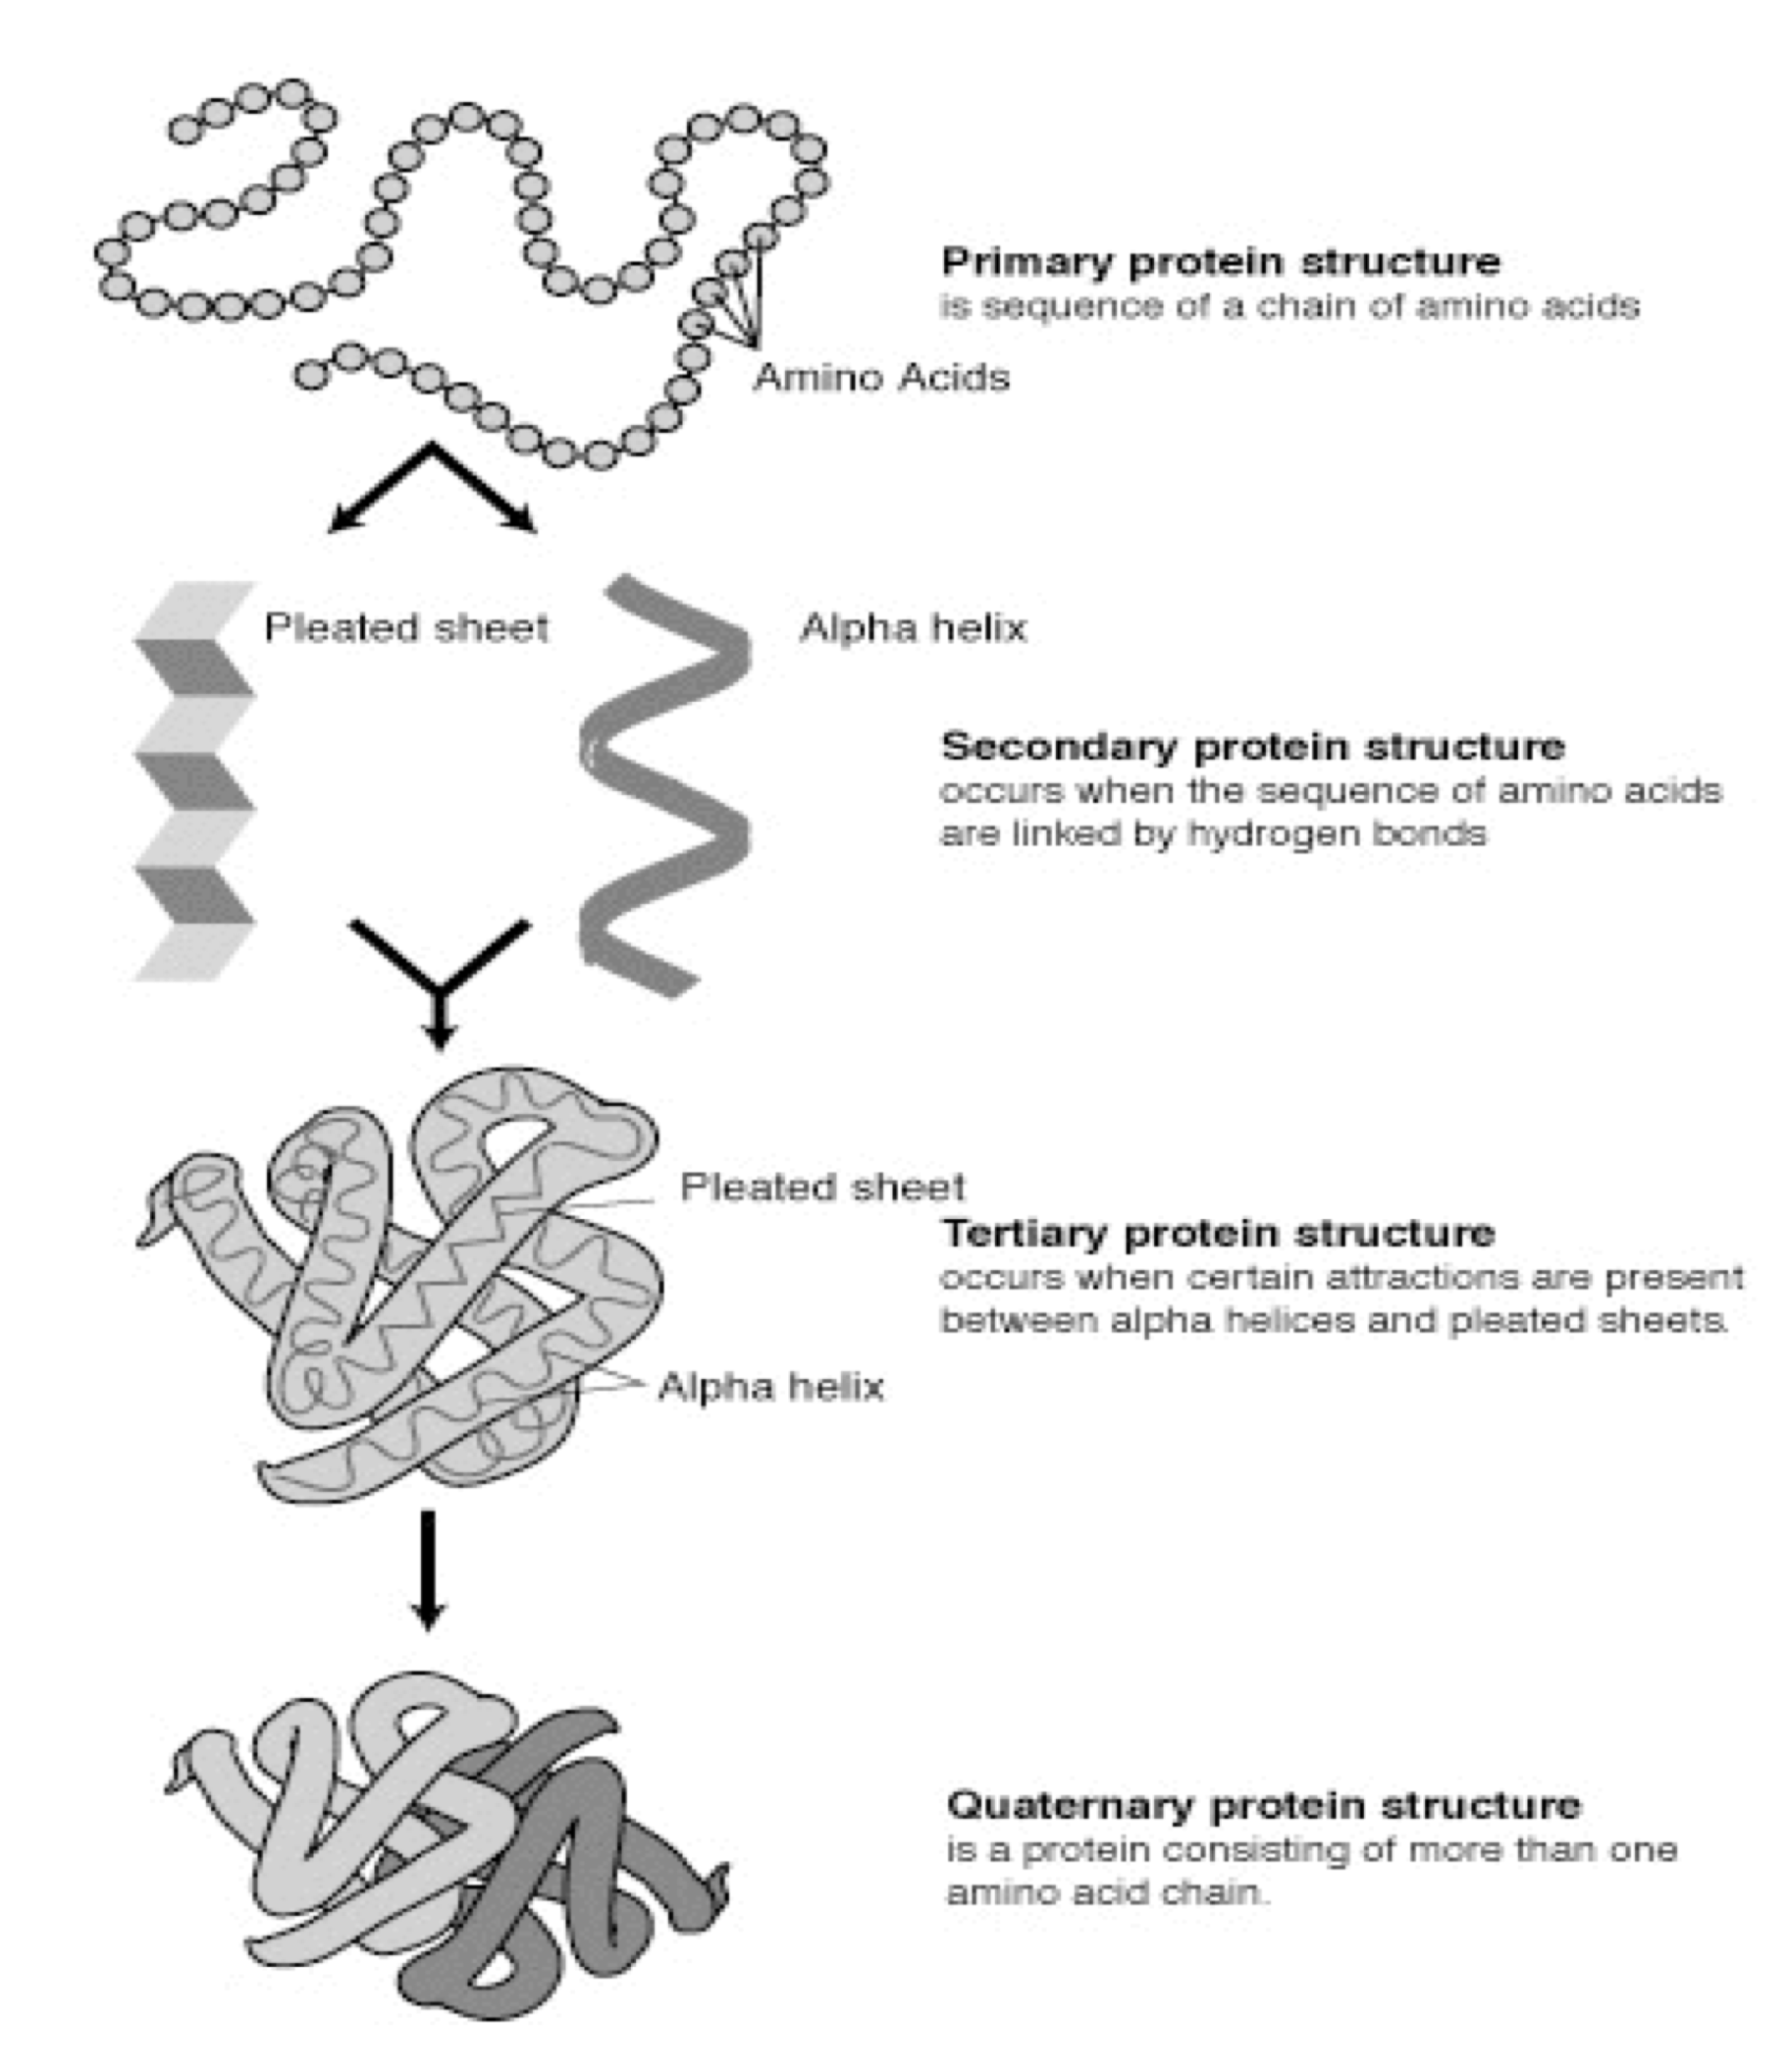
\includegraphics[width=0.5\textwidth]{figures/Proteine.png}
\end{center}
\paragraph{La struttura 3D di una proteina è molto complessa} La determinazione della
struttura 3D di proteine è un settore di ricerca molto attivo,
come mostra la crescita esponenziale di strutture depositate nel Protein Data Bank.\\
\section{Il cosmo "omico"}
\subsection{La genomica} 
\begin{itemize}
    \item \underline{Genoma:} Insieme dei geni di un organismo.
    \item \underline{Genomica:} scienza che se ne
    occupa.
    \item \underline{Genoma Umano:} Sequenziato
    completamente nel 2003.
    \item \underline{Occorre localizzare:} Elementi
    Funzionali:
    \subitem{-} Regioni 'utili' → geni;
    \subitem{-} Sequenze codificanti,
    comprendere i meccanismi che
    regolano l'espressione, scoprire
    la funzione, e cercare
    d'intervenire specificamente su
    quest'ultima.
\end{itemize}
Il costo del sequenziamento del genoma oggi è alla portata di ciascun individuo.
\subsection{Trascrittomica}
\begin{itemize}
    \item \underline{Trascrittoma:} l'insieme di tutti i
    trascritti (RNA messaggeri,
    mRNA)
    \item \underline{Trascrittomica:} scienza che se ne
    occupa.
    \item \underline{Occorre localizzare:} Profili di
    espressione:
    \subitem{-} più dinamico del genoma
    \subitem{-} microarrays monitorano i
    livelli di espressione di migliaia
    di geni allo stesso tempo.
    Mirano ad individuare
    correlazioni e legami tra
    espressione genica, attivazione
    e inibizione.
    Esempi: studio nella
    differenziazione di cellule
    staminali o evoluzione di
    tumori.
\end{itemize}
\subsection{Proteomica}
\begin{itemize}
    \item \underline{Proteoma:} l'insieme di tutte le
    proteine in un sistema biologico o
    nel suo genoma
    \item \underline{Proteomica:} scienza che se ne
    occupa.
    \item \underline{Occorre localizzare:} sia le
    proteine codificate dai geni che le
    possibili modificazioni post-
    traduzionali (gruppi prostetici,
    multidomini, fosforilazione, ecc).
    \item Alcune tecniche
    \subitem{-} Gel:
        \subsubitem 1° dimensione punto
        isoelettrico
        \subsubitem 2° massa molecolare
    \subitem{-} Spettrometria di massa:
    identifica una proteina in base
    al suo rapporto massa/carica in
    seguito a ionizzazione
\end{itemize}
\subsection{Genomica Strutturale}
\begin{itemize}
    \item \underline{Genomica strutturale:}
    determinazione della struttura
    terziaria e quaternaria (3D e
    domini) delle proteine.
    \item \underline{Tecniche:} cristallografia, NMR,
    homology modeling, cryoEM
    (microscopia crioelettronica)
    + AlphaFold (basato su AI)
    \item La struttura terziaria di una
    proteina è essenziale per
    determinarne la funzione
\end{itemize}
\subsection{Farmaco-genomica}
\begin{itemize}
    \item \underline{Farmacogenomica}: mira a
    prevedere la reazione di ciascun
    individuo verso un principio attivo
    in base al suo genotipo.
    \item \underline{Obiettivo:} creare terapie
    farmacologiche personalizzate
    per ottimizzare il risultato
    minimizzando gli effetti
    collaterali.
    \item Esempio: previsione di gravi
    reazione avverse a Abacavir
    nella terapia dell'HIV
\end{itemize}
\section{L'evoluzione ed il confronto tra sequenze}
Un allele (variante di un gene presente contemporaneamente
nella popolazione) può essere generato, fissato o mutare nel
tempo.\\
\textbf{Uno degli obiettivi in senso lato della bioinformatica è
stabilire se l'analisi dell'informazione riguardo a due
oggetti biologici (e.g. geni o proteine) permette di stabilire
una relazione di OMOLOGIA, cioè di discendenza da un
antenato comune}
Due sequenze che vengono separate fisicamente (per speciazione,
duplicazione ecc.) non si scambiano piu' "informazione" ed evolvono
indipendentemente, accumulando mutazioni. Spetta a noi trovare i tratti
conservati dal comune antenato.\\
Un modo per muoversi in tal direzione è allineare le sequenze e determinare la
percentuale di identita' o sequence identity (s.i.) (rapporto, in \% tra il numero
dei amminoacidi/basi identici rispetto al totale) o comunque il grado di similitudine.
Di norma, sequenze nucleotidiche non correlate hanno una s.i. ~50\%; sequenze
amminoacidiche non correlate hanno una s.i. ~20\%. Se tali valori aumentano,
aumenta la probabilità che le sequenze siano omologhe. Ma tale indice dovrebbe
tener conto anche della lunghezza delle sequenze.
Una s.i. del 90\% fra due sequenze di 100 a.a. ha un significato diverso rispetto alla
stessa s.i. su sequenze di 30 a.a.
\textbf{Allineare due sequenze significa stabilire se tra esse sussiste una
relazione di omologia}
\begin{titlepage}
    \begin{center}
        \vspace*{1cm}
        \LARGE
        \textbf{Lezione 2: Basi di Dati Biologiche}
        
    \end{center}
\end{titlepage}
\setcounter{page}{10}
\section{Le Basi di Dati Biologiche}
Il concetto di informazione è strettamente connesso a quello di dato e di
struttura.
Il dato è un osservabile (insieme di numeri, caratteri, simboli…)
La struttura è l' organizzazione ordinata di dati che ne consente
l'apprendimento.\\
Una banca dati è l'insieme di dati elementari, omogenei,
ordinati e fruibili. In altre parole: è una collezione
organizzata di dati
Esempio: elenco telefonico. L'informazione è strutturata in campi (nome,
cognome ecc.). Ogni persona con i propri dati è un record.
I dati biologici necessitano di un'organizzazione. Primo tentativo:
Margaret Dayhoff (1925-1983): raccolse, nel 1965, le sequenze di
65 proteine (lavoro pioneristico per il tempo!)
Le tecniche di sequenziamento rapido ed i progetti \textit{-omici} hanno
prodotto una quantita' esplosiva di dati, anche di sequenze
L'avvento di Internet ha facilitato di gran lunga l'acquisizione e la
distribuzione dell'informazione biologica in banche dati.\\
\subsection{Introduzione}
\begin{itemize}
    \item Sono collezioni di dati:
        \subitem{-} strutturati
        \subitem{-} indicizzati
        \subitem{-} aggiornati
        \subitem{-} interconnessi
    \item I database biologici sono legati a strumenti per:
        \subitem{-} recuperare records al loro interno 
        \subitem{-} aggiornare il database
        \subitem{-} combinare le informazioni
    \item Ci sono 6 principali categorie di basi di dati biologiche:
        \subitem{-} basi di dati di sequenze
            \subsubitem DNA
            \subsubitem RNA
            \subsubitem Proteine
        \subitem{-} basi di dati per il mapping
            \subsubitem geni
            \subsubitem cromosomi
            \subsubitem \dots
        \subitem{-} Strutture3d (PDB)
        \subitem{-} Trascrittomica
        \subitem{-} Funzionali (KEGG)
        \subitem{-} Per la letteratura (PubMed), ontologies (GO), \dots
\end{itemize}
A gennaio di ogni anno il Nucleic Accids Research pubblica un Database Issue, a gennaio:
\begin{itemize}
    \item nel 2020 contiene 89 nuovi database e l'aggiornamento di 90 database
    \item classificati nelle seguenti categorie
        \subitem{-} Nucleotide Sequence Databases
        \subitem{-} RNA sequence databases
        \subitem{-} Protein sequence databases
        \subitem{-} Structure Databases
        \subitem{-} Genomics Databases (non-vertebrate)
        \subitem{-} Metabolic and Signaling Pathways
        \subitem{-} Human and other Vertebrate Genomes
        \subitem{-} Human Genes and Diseases
        \subitem{-} Microarray Data and other Gene Expression Databases
        \subitem{-} Proteomics Resources
        \subitem{-} Other Molecular Biology Databases
        \subitem{-} Organelle databases
        \subitem{-} Plant databases
        \subitem{-} Immunological databases
        \subitem{-} Cell biology
        \subitem{-} COVID-19 databases
\end{itemize}
Le banche dati si strutturano e si integrano per favorire lo studio del dogma centrale della biologia.
Tre enti al mondo sono i principali.
\begin{itemize}
    \item EMBL
    \item NCBI
    \item DDBJ
\end{itemize}
Integrando collegamenti esterni (Swiss-prot, ExPASy,
UCSC, ecc, ecc…) sono un punto ideale di partenza.
\subsection{Dati di Sequenza}
Che dati si possono trovare?
\begin{itemize}
    \item Principalmente sono presenti
        \subitem{-} sequenze di caratteri (nucleotidi, amminoacidi)
        \subitem{-} o strutture
    \item L'uso della rappresentazione dei dati biologici di
    varia natura come sequenze è la forma di gran lunga
    più diffusa.
    \item Sequenze di DNA: formate da 4 tipi di lettere (a,c,g,t), convenzionalmente minuscole
    \item Sequenze di RNA: formate da 4 tipi di lettere (A,C,G,U), convenzionalmente maiuscole
    \item Sequenze proteiche: formate da 20 lettere (A, C, D, E, F, G, H, I,K, L, M, N, P, Q, R, S, T, V, W, Y), convenzionalmente maiuscole
\end{itemize}
Il formato FASTA-Pearrson: 
\begin{itemize}
    \item Rappresentazione mediante testo di sequenze nucleotidiche o
    peptidiche (lettere MAIUSCOLE).
    \item La prima riga (di lunghezza arbitraria) è preceduta da ">" e rappresenta
    la descrizione della sequenza.
    \item Le linee precedute da ">" o ";" sono considerate di commento e non
    vengono interpretate come dato di sequenza
    \item Le linee successive (ciascuna di 80 caratteri) rappresentano la
    sequenza.
    \item Un file fasta può avere estensione (non c'è uno standard)
\end{itemize}
Il formato XML (eXtensible Markup Language).
\begin{itemize}
    \item Replica la struttura logica del record nella banca dati
    \item I tag permettono di delimitare e definire campi e sottocampi
\end{itemize}

\section{NCBI}
NCBI (National Center for Biotechnology Information) presso il National Institute of Health. Offre accesso a tante risorse di vario tipo:
\begin{itemize}
    \item Sequenze geniche e proteiche
    \item Strutture terziarie
    \item Genomi completi
    \item Pathways
    \item EST (expressed sequence tags)
    \item Profili trascrittomici
    \item Cataloghi tassonomici
\end{itemize}
Fornisce accesso a numerosi database attraverso il sistema Entrez:
\begin{itemize}
    \item GenBank
    \item Swissprot
    \item PubMed
    \item GEO 
    \item \dots
\end{itemize}
Fornisce accesso anche a diversi software bioinformatici.
\subsection{Com'è strutturato il database}
Una ricerca qualunque dall'home page apre ENTREZ,
interfaccia per l'accesso ai database presenti in NCBI.\\
\begin{itemize}
    \item PubMed è l'interfaccia di accesso a
    MEDLINE.
    Con I suoi
    \subitem{-} 20 milioni di record fino agli anni '50
    \subitem{-} 4600 riviste da più di 70 paesi\\
    È la banca dati per la letteratura
    biomedica più completa.
    (Accessibile anche tramite EBI tramite 17 CiteXplore)
    \item Nucleotide è un database che
    raccoglie sequenze da diversi altri
    database di NCBI.
    Per sequenze nucleotidiche
    \subitem{-} EST ( expressed sequence tag )
    \subitem{-} GSS ( genome sequence surveys
    Gene è orientato ai geni, ai loci
    altre sequenze, B act A rtif C hromosome ,
    Y east A rtif C hromosome ,\dots)\\
    Inoltre:
    \subitem{-} RefSeq ( sistema di
    identificazione )
    \subitem{-} Unigene ( sequenze raggruppate )
    \subitem{-} UniProt ( proteine )
    \item Gene è orientato ai geni, ai loci
    \item Proteins è la sezione focalizzata sulle
    proteine, alle quali possono
    corrispondere strutture
    \item PubChem dedicato ai composti chimici
    \item In Genome genomi completi con riferimenti alla
    ricerca effettuata, varianti genomiche,
    ecc
    \item Informazioni su profili di espressione
    genica in diverse condizioni, modifiche
    post-traduzionali
    GEO (Gene Expression Omnibus)
    repository
\end{itemize}
GenBank è la banca dati di tutte le sequenze in NCBI (sincronizzata con
EMBL e DDBJ). Le sequenze derivano da diverse fonti e tipi:
\begin{itemize}
    \item Geni (regioni di regolazione, esoni, introni: unità ereditarie)
    \item EST (Expressed Sequence Tags)
    brevi segmenti di DNA trascritti e sequenz. da cDNA (ottenuto da
    mRNA retrotrascritto)
    \item STS (sequence tagged site, dove l'informazione genetica è mappata
    fisicamente)
    \item GSS (Genome Survey Sequence, vettori sequenze solo parzialmente sequenziate)
    \item HTGS (High Throughput Genomic Sequence, sequenze prodotte da tecniche di
    seconda generazione per il sequenziamento veloce, messe qui in “preview”)
    \item Sequenze di proteine (sezione nr, non redundant)
\end{itemize}
Così tanto materiale ha provocato l'esigenza di ordine: \textbf{RefSeq}.\\
RefSeq è stato ideato per far corrispondere a ciascun trascritto
normalmente prodotto da un gene e a ciascuna proteina una sequenza di
riferimento, un identificatore (accession number).\\
Altri esempi di identificatori NON RefSeq sono:
\begin{itemize}
    \item X02775 GenBank/EMBL/DDBJ nucleotidic sequence
    \item Rs7079946 dbSNP (single nucleotide polymorphism)
    \item N91759.1 An expressed sequence tag
    \item AAC02945 GenBank protein
    \item Q28369 SwissProt protein
    \item 1KT7 Protein Data Bank structure record
\end{itemize}
Refseq fornisce un identificatore per la sequenza di riferimento, curato dal
personale dell'NCBI.\\
formati principali degli id RefSeq sono:
\begin{itemize}
    \item Complete genome/chromosome/plasmid N\textbf{C}$\_\#\#\#\#\#\#$
    \item Genomic contig (segmenti sovrapposti di DNA segments che rappresentano una sequenza consenso) N\textbf{T}$\_\#\#\#\#\#\#$
    \item mRNA (DNA format) N\textbf{M}$\_\#\#\#\#\#\#$
    \item Protein N\textbf{P}$\_\#\#\#\#\#\#$
\end{itemize}
\paragraph{Un primo esempio di ricerca - L'Emoglobina}
Una delle prime proteine ad essere studiata (anni '30 e '40, da Mulder, Liebing et al.).\\
È stata la prima proteina ad essere usata negli allineamenti multipli di sequenza:
voglio fare dei confronti di sequenze (ad esempio per confrontare la stessa proteina prodotta da diverse specie). Con le prime tecniche di sequenziamento abbiamo scoperto che è stata localizzata in due loci, uno sul cromosoma 16 (subunità alfa) e 11 (subunità beta). I due geni sono regolati sia in base all'età che in base ai diversi tessuti.\\
È quindi un problema complesso che ha poi originato una serie di considerazioni.
La mioglobina, una globina (struttura globulare a 8 eliche)
che lega l'ossigeno nei tessuti muscolari, è stata la prima
proteina la cui struttura tridimensionale è stata risolta
tramite cristallografia.\\
L'emoglobina è un tetramero (due catene alfa e due beta negli
adulti) è il principale trasportatore di ossigeno nei vertebrati.
Assieme alla mioglobina è stata usata nei primi studi sugli
allineamenti multipli.\\
Negli anni '80 con le prime tecniche di sequenziamento è stata
localizzata in due loci, uno sul cromosoma 16 (subunità alfa) e 11
(subunità beta). I due geni sono regolati sia in base all'età che in
base ai diversi tessuti.
\subsubsection*{Ricerca dell'emoglobina}
\begin{enumerate}
    \item Inseriamo "beta globin" nella barra di ricerca
    \item Seguiamo poi il link a "Gene"
    \item Entrez Gene (ex LocusLink) è un portale curato che descrive loci genetici
        \subitem{-} nomenclatura
        \subitem{-} alias
        \subitem{-} accession numbers
        \subitem{-} fenotipi
        \subitem{-} OMIM (ereditarietà dei caratteri)
        \subitem{-} HomoloGene
        \subitem{-} mappatura sul genoma
        \subitem{-} collegamenti esterni
    \item In generale ad oggi quesa ricerca trova 126 entries
    \item Intestazione: Entrez Gene, Noa: "Official Symbol", HBB per la beta globina
    \item Limitiamoci alla ricerca per Homo Sapiens (selezionando sulla destra da Results by taxon)
    \item Cliccando la specie si aggiorna automaticmente la stringa di ricerca: {\ttfamily(beta globin) AND "Homo sapiens" [ porgn:\_txid9606 ]}
    \item Con il limite Homo Sapiend le entries sono solo 41
    \item Apriamo la prima entry
    \item Sulla dx in basso troviamo numerosi link a database esterni
    \item Abbiamo una sezione sulle regioni genomiche, una sulla bibliografia
    \item Sezione interessante: GeneRif (intended to facilitate access to publications documenting experiments that add to our understanding of a gene and its function)
    \item E ancora Fenotipi, Variazione Genica, Pathways per Biosistemi e Interazioni note con altri geni.
    \item Ontologia: (fondamentale per sistemi automatici di apprendimento). Classificazione
    e organizzazione dei dati in categorie predefinite così da agevolare l'individuazione di
    analogie e caratteristiche primarie. Può essere di diversi tipi, ma la principale distingue:
        \subitem{-} Funzione molecolare
        \subitem{-} Localizzazione cellulare
        \subitem{-} Processo biologico
    \item Catalogazione RefSeq (a fine pagina)
\end{enumerate}
\subsection{Operatori Booleani}
\subsubsection{Operatore AND (\&)}
Restringe il campo di ricerca, inserendo ad es. la stringa:
{\ttfamily equus caballus AND hemoglobin alpha}\\
La banca dati ci mostrerà una lista di sequenze proteiche i cui campi di
descrizione contengono entrambe le parole. Quindi le sequenze proteiche
del cavallo che non contengono nella descrizione la parola hemoglobin
non vengono selezionate.
\subsubsection{Operatore OR (|)}
Estende il campo di ricerca, digitando ad esempio:
Restringe il campo di ricerca, inserendo:
{\ttfamily homo sapiens OR mus musculus}\\
Otterremo una lista di sequenze i cui campi contengono la parola homo
sapiens o la parola mus musculus.
L'operatore allarga l'insieme
delle sequenze che incontrano le nostre esigenze.
\subsubsection{Operatore NOT (!)}
Restringe il campo di ricerca, inserendo:
{\ttfamily homo sapiens NOT hemoglobin}
Richiederemo sequenze i cui campi contengono la parola homo sapiens
ma non la parola hemoglobin.
\subsubsection{Combinazione di Operatori Booleani}
Gli operatori booleani si possono combinare, vengono letti da sinistra a
destra. Per questo sono utili le parentesi. Ad esempio: globin AND promoter OR enhancer produce quasi 5000
hits. Ma se si scrive globin AND (promoter OR enhancer) se ne
ottengono circa 70.\\
Altre possibilità sono:
\begin{itemize}
    \item Specificare un organismo (human, nella query:
    human[ORGN]
    \item Usare l'asterisco: glob * restituisce tutte le entry che
    contengono una stringa che inizia per “glob”
    \item Usare le virgolette “” . La ricerca di “toxin B1” restituirà le
    entries che contengono esattamente la stringa intera.
    \item \dots
\end{itemize}
\subsection{Nel dettaglio}
\paragraph{Homologene}
la risorsa ideale per individuare gruppi
di geni omologhi negli eucarioti presenti in NCBI
\paragraph{OMIM}
Catalogo di geni umani e disordini genetici
\paragraph{SNP}
Single Nucleotide Polimorfism
\newpage
\section{Proteine - Le banche dati proteiche più usate}
\paragraph{Uniprot}
(Universal Protein Resource) raccoglie le informazioni dei database:
\begin{enumerate}
    \item Swiss-prot (SIB)
    \item TrEMBL (EBI) 
    \item PIR
\end{enumerate} 
Offre la possibilità di effettuare Text
Search o Blast Search. Viene curato anche un database NON RIDONDANTE
(UniRef).
\paragraph{Swissprot}
Molto curato e detagliato, con annotazioni circa funzione, struttura, modificazione e altre informazioni utili.
\paragraph{TrEMBL}
È la traduzione in silico di ogni entry codificante del database primario dell'EMBL, non è accurato, ma è ricchissimo.
\paragraph{PIR}
È il discendente diretto del database della Dayhoff, è curato a mano e le annotazioni sono molto ricche e precise.
\subsection{NCBI Protein - non molto ricco}
Entrez Protein: Contiene diverse informazioni su proteine
\begin{itemize}
    \item 147 amminoacidi
    \item PRI: primates
    \item $NP\_000509$ (protein accession number)
    \item $NM\_000518.4$ (mRNA, RefSeq)
    \item Riferimenti bibliografici
    \item Sequenze FASTA (Opzione Display)
    \item Siti di modificazione post-traduzionale (AA94, AA121)
    \item Riferimenti ad altri database
    \item Sequenza amminoacidica (1 lettera)
\end{itemize}
È un record non molto ricco dal punto di vista dei dati delle proteine.
\subsection{Uniprot}
Uniprot è il più completo database centralizzato per le sequenze proteiche.\\
È organizzato su 3 livelli:
\begin{enumerate}
    \item Uniprot Knowledge Base
        \subitem{-} Swiss-Prot (curato)
        \subitem{-} TrEMBL (automatico)
    \item UniProt Reference
    clusters (UniRef)
        \subitem{-} Cluster di proteine che
        condividono il 50\%, 90\%,
        100\% di identità di
        sequenza
    \item UniProt Archive (UniParc)
        \subitem{-} Archivio di sequenze
        proteiche stabile, non
        ridondante, da diverse 58 fonti
\end{enumerate}
\subsubsection{Struttura del database}
Nella homepage abbiamo la classica barra di ricerca e subito sotto i link di accesso alle diverse informazioni contenute in Uniprot.\\
\paragraph{Un esempio di ricerca}
\begin{enumerate}
    \item Inseriamo "{\ttfamily hbb}" nella barra di ricerca.
    \item Sulla sinistra possiamo selezionare gli organismi a cui restringere la ricerca. Selezioniamo Humans.
    \item Questo aggiornerà automaticamente la stringa di ricerca: {\ttfamily hbb AND organism: "Homo sapiens (Human) [9605]"}
    \item Selezioniamo la prima entry.
    \item Sulla sinistra troviamo la tavola con tutti i contenuti disponibili.
    \item Tra i più importanti abbiamo: "Function" (che specifica la funzione della proteina), "Pathology \& Biotech", "Expression", "Interaction", "Family \& Domains", \dots
    \item In "Structure" e altre sezioni troviamo i link a PDB (Protein Data Bank), database di strutture proteiche.
    \item In "Sequence" troviamo tutta la sequenza proteica, scaricabile in formato FASTA.
    \item Abbiamo inoltre vari link di collegamento ad altri database di sequenze (EMBL,GeneBank, DDBJ), varianti, \dots
\end{enumerate}
\subsection{ExPASy}
(Expert Protein Analysis System)\\
È una risorsa curata, espressione del SIB (Swiss Institute of
Bioinformatics). Principalmente dedicata alle proteine.\\
La risorsa principale che ha prodotto è SwissProt (confluita in Uniprot). Rimane un punto di riferimento per molti tools. 

\begin{titlepage}
    \begin{center}
        \vspace*{1cm}
        \LARGE
        \textbf{Lezione 3: Allineamenti di Sequenze - concetti e algoritmi}

    \end{center}
\end{titlepage}
\setcounter{page}{19}
\section{Allineamenti di Sequenze}
Un primo e precoce allineamento di sequenze si ha nel 1961: H.C. Watson and J.C. Kendrew,
“Comparison Between the Amino-Acid Sequences of Sperm Whale Myoglobin and of Human Hæmoglobin.” Nature 190:670-672, 1961.\\
\paragraph{L'allineamento di sequenze a coppie è un'operazione fondamentale in bioinformatica}
È utilizzato per decidere se due proteine (o geni) sono correlate strutturalmente e funzionalmente.\\
Viene utilizzato per identificare i domini o motivi che sono
condivisi tra le proteine. È alla base della ricerca con BLAST (prossime lezioni) e viene utilizzato anche per l'analisi dei genomi.
\paragraph{Allineamento a coppie: sequenze di proteine possono essere più informative del DNA}
Le proteine sono più informative del DNA (20 vs 4 caratteri);
molti aminoacidi condividono proprietà biofisiche.\\
Ricordiamo che i codoni sono degenerati: i cambiamenti in terza posizione
spesso non alterano l'amminoacido che ne è specificato
(mutazioni sinonime). Le sequenze di proteine offrono un più lungo tempo di
"look-back" e le sequenze di DNA possono essere tradotte in proteine,
e poi utilizzate negli allineamenti a coppie.
\subsection{Definizione - \underline{Allineamento a coppie}}
Il processo che allinea due sequenze per
raggiungere livelli massimi di identità (e
conservazione, nel caso di sequenze di
amminoacidi) al fine di valutare il grado di
similitudine e la possibilità di omologia.
\subsection{Altre definizioni}
\begin{itemize}
    \item \underline{\textbf{Identità}}
        \subitem La misura in cui due sequenze (di nucleotidi o aminoacidi) sono
        invarianti. (es. identità del 32\% => 32 a.a. su 100 sono
        ordinatamente identici)
    \item \underline{\textbf{Conservazione}}
        \subitem In una sequenza, modifiche in una specifica posizione di un
        amminoacido (o meno comunemente, di un nucleotide) che
        preservano le proprietà fisico-chimiche del residuo originale.
    \item \underline{\textbf{Similitudine}}
        \subitem La misura in cui due sequenze (di nucleotidi o aminoacidi)
        sono correlate. Si basa su identità + conservazione.
    \item \underline{\textbf{Omologia}}
        \subitem Similitudine attribuita a discendenti da un
        antenato comune.
        \subitem{!} \textbf{Nota bene:}
            \subsubitem{-} OMOLOGIA indica che due entità (es. 2 sequenze) hanno
            una stessa origine filogenetica, cioè derivano da un antenato
            comune. È un carattere QUALITATIVO.
            \subsubitem{-} SIMILITUDINE indica che due entità (es. 2 sequenze), in
            relazione ad un certo criterio comparativo, hanno un certo
            grado di similitudine. È un carattere QUANTITATIVO
            (vedremo tra breve come definirla).
        \subitem{!} \textbf{Osservazioni:}
            \subsubitem{-} La struttura di una proteina dipende della sua sequenza di a.a. (concetto alla
            base del Protein Folding).
            \subsubitem{-} La struttura determina la funzione molecolare della proteina.
            \subsubitem{-} Se una sequenza proteica è conservata durante l'evoluzione ed è quindi
            presente in organismi diversi (famiglia di proteine) è ragionevole assumere che le
            funzioni che svolge siano simili o per lo meno correlate.
        \subitem{!} \textbf{Passi per predizione di funzione:}
            \begin{enumerate}
                \item Identificazione delle proteine di una famiglia (evolute da un
                progenitore comune $\rightarrow$ sequenza di a.a. abbastanza simile.)
                \item dentificazione degli a.a. che svolgono un ruolo strutturale o
                funzionale analogo (allineamento).
            \end{enumerate}
\end{itemize}
\paragraph{Esempio 1:} la catena $\beta$ dell'emoglobina e miogobina «si somigliano» 
\begin{center}
    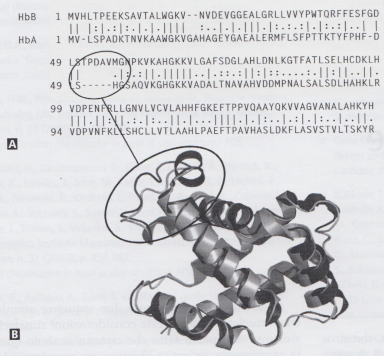
\includegraphics[width=0.5\textwidth]{figures/globine.png}
    \captionof{figure}{Le zone con indel nelle sequenze sono strutturalmente dissimili}
\end{center}
\begin{itemize}
    \item \underline{\textbf{Ortologhi}}
        \subitem Sequenze omologhe in diverse specie che derivano,
        tramite la speciazione, da un gene ancestrale
        comune. La funzione può essere o non essere
        simile.
    \item \underline{\textbf{Paraloghi}}
        \subitem Sequenze omologhe all'interno di una singola specie
        sorte dalla duplicazione genica.
\end{itemize}
\begin{center}
    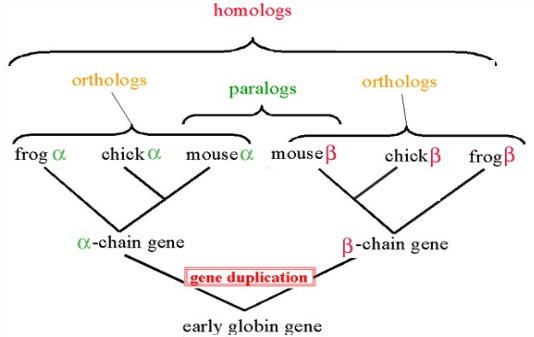
\includegraphics[width=0.5\textwidth]{figures/ortpar.png}
    \captionof{figure}{Ortologhi e paraloghi sono spesso rappresentati in un albero singolo.}
\end{center}
\newpage
Ortologhi: membri di una famiglia di geni (proteine) in vari organismi.
\begin{center}
    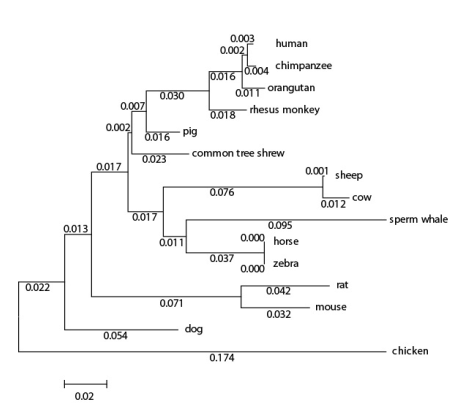
\includegraphics[width=0.5\textwidth]{figures/ortpar2.png}
    \captionof{figure}{Questo albero mostra gli ortologhi della globina.}
\end{center}
Paraloghi: i membri di una famiglia di geni (proteine) all'interno di una specie.
\begin{center}
    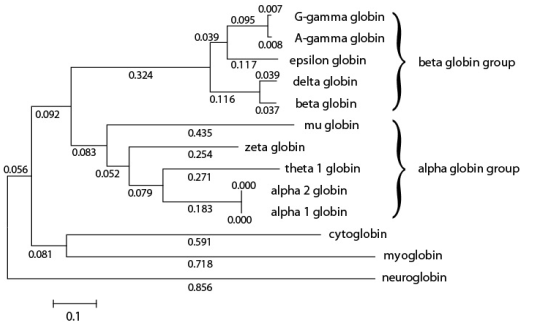
\includegraphics[width=0.5\textwidth]{figures/ortpar3.png}
    \captionof{figure}{Questo albero mostra i paraloghi della globina umana.}
\end{center}
\section{Confrontare due sequenze}
\paragraph{Come posso trasformare una stringa in un'altra?} 
Un modo semplice per capirlo è allineare le due stringhe:\\
ESEMPIO: 1 - LA CASA NUOVA; 2 - LA CASSA VUOTA\\
\begin{center}
    1 - L A C A - S A N U O V A\\
    2 - L A C A S S A V U O T A\\
    oppure\\
    1 - L A C A - S A - N U O V A\\
    2 - L A C A S S A V - U O T A\\
\end{center}
Nel secondo caso c'è un'operazione in più. 
\begin{itemize}
    \item Il numero minimo di operazioni necessarie per allineare
    due sequenze ne misura la distanza.
    \item La Natura dispone di varie operazioni per trasformare un
    oggetto nell'altro (mutazioni, indel…)
    \item L'evoluzione sceglie la via piu' breve (principio di
    massima parsimonia); cio' si manifesta tramite l'analisi
    dell'allineamento.
\end{itemize}
Dobbiamo avere chiari i concetti di match (residui
appaiati), mismatch (sostituzioni) e gap (indel).
\subsection{Come identificare le zone di somiglianza locale tra due sequenze?}
\subsubsection{Matrice a punti - dot plot}
È un modo relativamente semplice.\\
Confrontiamo la stringa con se stessa (autoconfronto):
\begin{enumerate}
    \item Mettiamo una x per ogni identità
\end{enumerate}
\begin{center}
    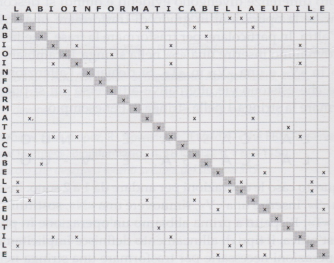
\includegraphics[width=0.5\textwidth]{figures/autoconfronto.png}
    \captionof{figure}{\dots piuttosto banale. Cambiamo la seconda stringa.}
\end{center}
Effettuiamo un'inversione. Il pattern delle diagonali lo
mostra chiaramente: la diagonale principale si spezza ma
porzioni delle stringhe sono identiche.
\begin{center}
    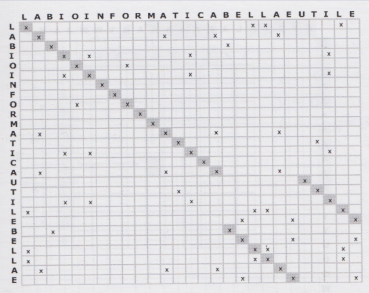
\includegraphics[width=0.5\textwidth]{figures/inversione.png}
\end{center}
Possiamo individuare facilmente alcuni patterns mediante le matrici a punti (la prima stringa in alto resta immutata):
\begin{itemize}
    \item Inversione di parole\\
    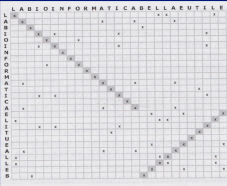
\includegraphics[width=0.3\textwidth]{figures/inv2.png}
    \item Ripetizione di parole\\
    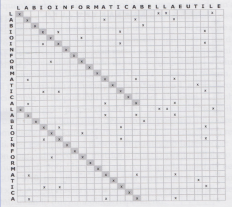
\includegraphics[width=0.3\textwidth]{figures/rip.png}
    \item Delezione di caratteri\\
    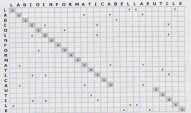
\includegraphics[width=0.3\textwidth]{figures/del.png}
\end{itemize}
Se però allineamo sequenze di acidi nucleici (solo 4 lettere) il “segnale” di similitudine è mascherato dal grande rumore di fondo. Servono FILTRI per ridurre il rumore.
\paragraph{Una semplice osservazione:}le zone delle sequenze più simili
localmente si distribuiscono su diagonali; le altre somiglianze puntiformi si distribuiscono casualmente.
Allora, è meglio confrontare le sequenze non per singole posizioni, ma per interi segmenti (FINESTRE).\\
Potremmo usare delle finestre scorrevoli.\\
ESEMPIO: confrontiamo una finestra di 5 residui in una seq
con una finestra di 5 residui nell'altra. Confronto tutte le
finestre (facendole scorrere), e metto una * al centro della
finestra solo se ho un match totale.
\begin{center}
    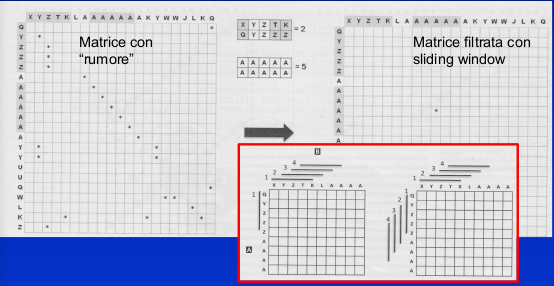
\includegraphics[width=0.5\textwidth]{figures/sliding.png}
\end{center}
In generale: si fa scorrere una finestra alla volta.
\paragraph{La procedura}
\begin{enumerate}
    \item Definiamo la posizione di una casella $(x,y)$.
    \item Fissiamo il centro della finestra, di raggio $g$.
    \item La lunghezza della finestra è dunque: $L= 2g+1$
    \item Il numero $N$ di residui identici in quella finestra è allora: $N(x,y) = \sum^{+g}_{h=-g} S(x + h, y+h)$
        \subitem $S=1$ se il carattere in $x+h$ è identico a quello in $y+h$; altrimenti $S=0$
\end{enumerate}
Questa regola è però molto restrittiva. A noi interessa anche
la similitudine, non solo l'identità. Potremmo definire una soglia $s$, per cui:
\begin{itemize}
    \item Se $N(x,y)>s$ mette un simbolo nella casella in posizione $x,y$.
\end{itemize}
Dobbiamo quindi misurare la similitudine, e.g. tra aa o basi. Un
esempio di matrice di punteggio (non di punti!!) per seq
di nucleotidi può essere:
\begin{center}
    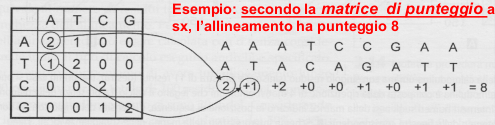
\includegraphics[width=0.5\textwidth]{figures/mat.png}
\end{center}
Misurata la similitudine, possiamo allora attribuire un nuovo punteggio al confronto fra due finestre:
\begin{itemize}
    \item Se $N(x,y)$ è il numero dei residui simili, ed è la media dei punteggi
    delle singole coppie prelevati dalla matrice di punteggio scelta:
    \item $N(x,y) = \sum^{+g}_{h=-g} {S(x + h, y+h)\over L}$
\end{itemize}
$S$ ora dipende da quale matrice di punteggio scegliamo e dalla
lunghezza della finestra. Possiamo quindi essere un po' più "elastici" pur mantenendo
la regola:
\begin{itemize}
    \item Se $N(x,y)>s$ mette un simbolo nella casella in posizione $x,y$.
\end{itemize}
$s$ lo decide la matrice di punteggio (cioè la similitudine).
\subsubsection{In breve}
In conclusione, la visualizzazione (ed il calcolo) di una
matrice a punti dipende da:
\begin{enumerate}
    \item La lunghezza $L$ della finestra scorrevole scelta
    \item Il metodo per misurare la similitudine $S(x,y)$
    \item La soglia $s$ per “marcare” la casella rispettiva
\end{enumerate}
In pratica conviene fissare 2 parametri e variare il terzo per rendere le zone di
similitudine più evidenti. Molti programmi fanno questo.\\
Es. DOTTER/Dotlet - assegna un colore dipendentemente da $S$.
\paragraph{Nota:}Analogamente all'identità di sequenza, che si può
misurare in percentuale (\%), anche la similitudine, una volta
quantificata, si può misurare in \%.\\
$S_1$ e $S_2$ sono due sequenze lunghe, rispettivamente, $L_1$ ed $L_2$.\\
Scelta $L_1$ come riferimento si ha:
$$ SequenceIdentity(s.i.) = ({\#matches \over L_1}) * 100 $$
$$ SequenceSimilarity(s.s.) = ({S_1 vs. S_2 s.c. \over S_1 vs. S_2 i.c.}) * 100 $$
\textit{s.c. = similarity score, ed è ottenuto allineando $S_1$ con $S_2$, e attribuendo il punteggio ottenuto dalla matrice discore.\\i.c. = identity score ed è ottenuto allineando $S_1$ con sè stessa ed attribuendo il punteggio ottenuto dalla matrice di score}
\textit{\\Nota:} se sono presenti indel, a denominatore metto la lunghezza
dell'allineamento (compresi gli indel), e non la lunghezza originale della sequenza.
\section{Algoritmi dinamici di allineamento}
I dot plots non tengono in considerazione gli indel. Occorrono altri
algoritmi che, passo a passo e seguendo una certa direzione, trovino
l'allineamento con:
\begin{itemize}
    \item Maggior numero di simboli identici
    \item Minor numero di indel (sfavorite evolutivamente)
\end{itemize}
Esempio: proviamo tutte le combinazioni da sx a dx, riempiendo una colonna alla volta (qui mostriamo solo i primi 3 residui!!)\\
Stabiliamo inoltre i punteggi:
\begin{itemize}
    \item -1 per indel
    \item 0 per residui diversi
    \item +1 per residui identici
\end{itemize}
Il numero delle combinazioni possibili è molto grande, specie per
sequenze lunghe. Nel 1970 NEEDLEMAN e WUNSCH creano un algoritmo, poi
migliorato ed esteso. Noi analizziamo l'originale.
\subsection{Il concetto}
distribuiamo le due sequenze in una matrice. Il possibile
allineamento tra le due identifica un percorso che unisce le caselle dei
residui appaiati.
\begin{center}
    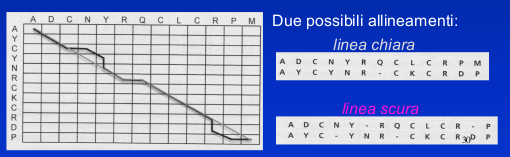
\includegraphics[width=0.5\textwidth]{figures/algo.png}
\end{center}
\subsection{Regole pratiche}
\begin{enumerate}
    \item Il percorso ha una direzione e procede solo in avanti (NON si torna indietro!)
    \item Occorre trovare il percorso con il \textbf{maggior} numero di aa identici e il \textbf{minor} numero di indel
    \item Occorre anche tener conto della similitudine fra amminoacidi (significato evolutivo)
    \item IMPORTANTE: un allineamento ottimale è sempre
    composto da suballineamenti ottimali (cioè: togliendo uno
    ad uno i residui dal fondo, l'allineamento deve restare
    ottimale, per poter ricostruire il percorso a ritroso)
\end{enumerate}
\subsection{Step}
\begin{enumerate}
    \item INIZIALIZZAZIONE della matrice: regola molto semplice; 1
    se identici, 0 altrimenti. N.B. ora $(x,y)$ identifica: (residuo in
    colonna, residuo in riga) (N.B. dopo aver trattato le matrici
    di score potremo normalizzare diversamente)\\
    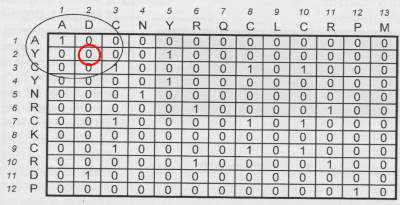
\includegraphics[width=0.6\textwidth]{figures/init.png}
    \item Partiamo da (1,1) (in alto a sx:
    la direzione è importante!!):
    (1,1) $\rightarrow$ (2,2)
    L'unico percorso possibile è
    questo: per “ricordarmelo”
    sommo il valore della cella
    (1,1) a quello della cella (2,2)
    da matrice inizializzata
    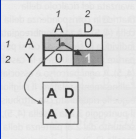
\includegraphics[width=0.3\textwidth]{figures/due.png}
    \item Prossimo step: verso (2,3). Ci sono due possibili percorsi, corrispondenti a due diversi
    allineamenti: scelgo quello con punteggio finale maggiore, sempre sommando casella precedente a (2,3)\\
    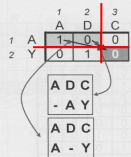
\includegraphics[width=0.3\textwidth]{figures/tre.png}
    \item Procediamo analogamente: ad esempio, verso (4,4)\\
    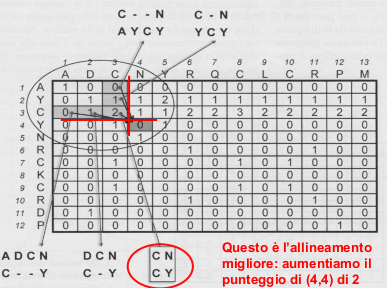
\includegraphics[width=0.6\textwidth]{figures/quattro.png}
    \item e oltre, ad es. verso (4,5): qui il nuovo punteggio sarà 3\\
    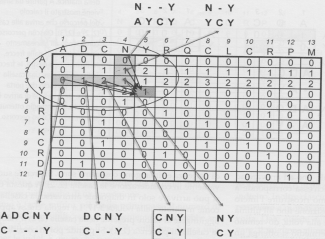
\includegraphics[width=0.6\textwidth]{figures/cinque.png}
    \item Alla fine arriveremo fino all'ultima casella in basso a dx:\\
    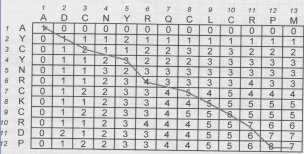
\includegraphics[width=0.6\textwidth]{figures/sei.png}
    \item Da essa possiamo spostarci a ritroso poiché abbiamo
    memorizzato i migliori punteggi dalle caselle precedenti.
    Abbiamo così determinato il miglior allineamento:\\
    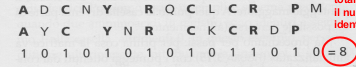
\includegraphics[width=0.8\textwidth]{figures/sette.png}
    \subitem \textit{Qui il punteggio totale coincide con il numero di residui
    identici.\\ ${8 \over 15} = 0.53 = 53\%$ identità di sequenza}
\end{enumerate}
\paragraph{In termini formali \dots} La casella (i,j) avrà lo score S(i,j)
ricalcolato a partire dalla matrice di inizializzazione in questo
modo:
\begin{center}
    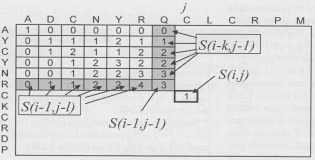
\includegraphics[width=0.6\textwidth]{figures/otto.png}
    $$ S(i,j) = {s(a,b) + max[S(i-1,j-1),S(i-k,j-1),S(i-1,j-l)]}$$
\end{center}
Dovremmo però trovare un modo più efficace di inizializzare la
matrice tenendo conto della similarità fra aa.
\subsection{Needleman-Wunsch: programmazione dinamica}
NW garantisce l'ottimalità dell'allineamento, anche se l'algoritmo non
calcola tutti i possibili allineamenti.
È un esempio di un algoritmo di programmazione dinamica:
un percorso ottimale (allineamento) è identificato dall'estensione
graduale di sottopercorsi localmente ottimali.
Dunque, una serie di decisioni è effettuata ad ogni passo
dell'allineamento per trovare la coppia di residui con il miglior
punteggio per quel passo.\\
L'algoritmo di Needleman-Wunsch è disponibile presso
EBI, che ospita molti tools per allineamenti locali e globali di
sequenze (Pairwise Sequence Alignment).

\begin{titlepage}
    \begin{center}
        \vspace*{1cm}
        \LARGE
        \textbf{Lezione 4: Allineamenti di Sequenze 2\\Matrici di Sostituzione}

    \end{center}
\end{titlepage}
\setcounter{page}{30}
\section{Waterman-Smith}
Un problema dell'algoritmo di Needleman-Wunsch: non si
tiene conto della penalizzazione delle indel.\\
L'algoritmo di WATERMAN-SMITH (1976) introduce
una funzione di penalizzazione delle indel, per migliorare
l'algoritmo NW, serve un sistema di pesatura delle indel, ad esempio:
$$ w(k) = g + e(k-1)$$
Il peso $w$ di una indel di lunghezza $k$ dipende dalla
penalizzazione per l'apertura di una singola indel ($g$) e
dalla penalizzazione per l'allungamento ($e$).
\subsection{L'algoritmo}
Nella pratica l'algoritmo procede in questo modo:
\begin{enumerate}
    \item nserisce una riga e una colonna 0-ime alla matrice
    di inizializzazione (calcolata ad esempio partire da
    BLOSUM o PAM che vedremo, ecco perché non ha
    solo 0 o 1). \\ Nella riga e colonna
    ombreggiate è
    sviluppata la funzione di
    penalizzazione: $w(k) = -12-4(k-1)$\\
    La riga e la colonna 0-sime contengono il
    punteggio che la
    sequenza avrebbe se
    allineata a una delezione
    lunga fino alla cella
    corrispondente.
    \item Tiene conto dei possibili modi per arrivare alla
    casella $(i,j)$. Il suo punteggio $S(i,j)$ dipende da essi:
    \begin{enumerate}
        \item Mi muovo in diagonale: no indel e
        punteggio dato da: punteggio
        della casella di partenza +
        punteggio della casella $(i,j)$
        secondo la matrice di
        inizializzazione (come in NW)
        \item Mi muovo in verticale o
        orizzontale: inserisco indel nella
        sequenza $i$ e $j$. Il punteggio sarà
        dato da: punteggio della casella
        di partenza - funzione di
        penalizzazione $w(k)$ ($k$ è la
        lunghezza della indel).
        \item Scelgo alla fine il percorso che dà
        il punteggio migliore
    \end{enumerate}
\end{enumerate}
\begin{center}
    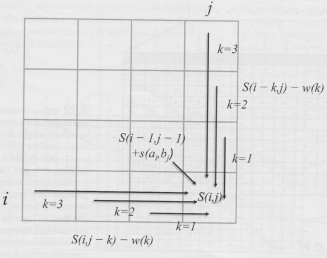
\includegraphics[width=0.5\textwidth]{figures/nw.png}
\end{center}
\section{Allineamento: globale vs locale}
\paragraph{Allineamento globale} (NW e SW visto finora) si estende da un
capo all'altro di ogni sequenza.
\paragraph{Allineamento locale} trova le regioni (sottosequenze) di due
sequenze che si allineano in modo ottimale.
\begin{center}
    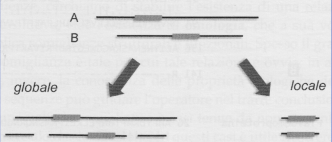
\includegraphics[width=0.5\textwidth]{figures/gl.png}\\
    \textit{Qui l'allineamento
    globale maschera la
    corrispondenza tra
    zone somiglianti}
\end{center}
SW si può modificare per renderlo capace di calcolare
allineamenti locali: basta introdurre fra i casi possibili $S(i,j)=0$ nel
caso in cui nell'allineamento globale fosse negativo
\paragraph{Esempio:} L'allineamento fra una
flavoemoproteina (con
un dominio di tipo
emoglobinico) e la
catena A
dell'emoglobina umana
\begin{itemize}
    \item \textbf{globale}: più difficile
    notare
    quantitativamente la
    similitudine
    \item \textbf{locale:} più apparente
\end{itemize}
\begin{center}
    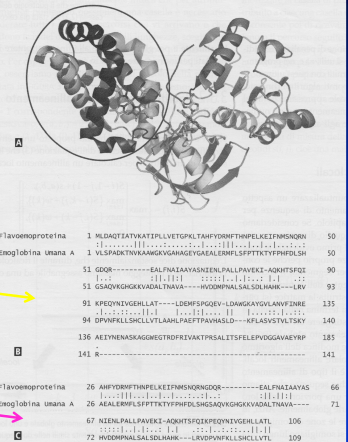
\includegraphics[width=0.5\textwidth]{figures/es1.png}\\
\end{center}
\paragraph{Esempio:} SW locale:dopo aver ricalcolato la matrice
cerco la cella con il valore massimo assoluto e parto da lì.\\
Gli stessi due peptidi di prima, allineati con Waterman-Smith
globale e locale danno luogo a matrici ed allineamenti
diversi. Partendo dalle caselle con score maggiore il
percorso a ritroso individua allineamenti differenti (non
sempre AL è sottoinsieme di AG)
\begin{center}
    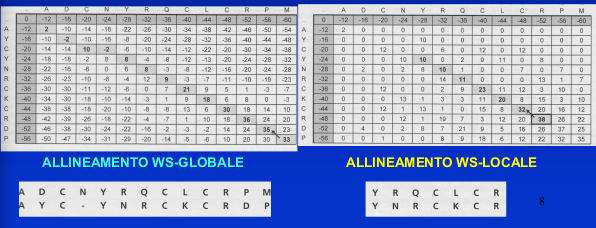
\includegraphics[width=0.5\textwidth]{figures/es2.png}\\
\end{center}
\subsubsection{In conclusione}
\begin{itemize}
    \item L'allineamento locale è quasi sempre utilizzato per il ricerche su
    database (tramite BLAST). E 'utile per trovare domini (o regioni
    limitate di omologia) all'interno di sequenze.
    \item Smith e Waterman (1981) hanno risolto il problema
    dell'allineamento locale ottimale di sequenze.
    \item Altri metodi (BLAST, FASTA) sono più veloci ma meno accurati.
    Li vedremo in seguito.
    \item In ogni caso, qualunque metodo di allineamento si scelga esso
    fornirà un punteggio S all'allineamento. Ricordiamo sempre che lo
    score S dipende dal metodo di allineamento e non è assoluto!
\end{itemize}
\subsection{Significatività statistica di un allineamento}
\paragraph{Domanda:}Ho allineato due sequenze A e B, ottenuto il punteggio S.
Come posso capire se sono omologhe? Che probabilità ho di
trovare il punteggio S “per caso”?\\
Il problema è più facilmente risolvibile per gli allineamenti
locali, e meno per quelli globali.
\subsubsection{Significatività allineamento globale: lo Z score}
La seq $A$ è mantenuta fissa; la $B$ è
“anagrammata” n volte ed ogni volta
globalmente allineata ad $A$, calcolando
lo score $S_i$ per l'allineamento $i$.
\begin{center}
    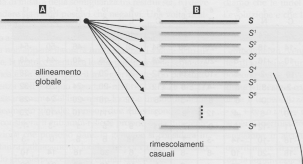
\includegraphics[width=0.5\textwidth]{figures/sig1.png}\\
\end{center}
$S_i$ si distribuisce su una curva di cui si
calcola la media $\mu$ e la deviazione
standard $\sigma$, Si definisce allora la
distanza $Z$ del punteggio $S$
dell'allineamento dalla media in termini
di dev. standard:
$$ Z = { S -\mu \over \sigma}$$
\begin{center}
    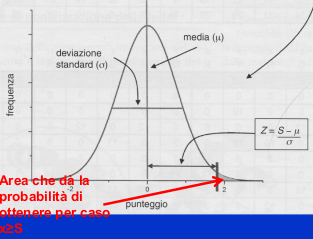
\includegraphics[width=0.5\textwidth]{figures/sig2.png}\\
\end{center}
\begin{center}
    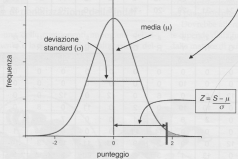
\includegraphics[width=0.5\textwidth]{figures/sig3.png}\\
\end{center}
\begin{itemize}
    \item Uno Z-score 0 = significa che la somiglianza osservata non è migliore
    rispetto alla media di permutazioni casuali della sequenza, e può anche
    essere casuale.
    \item Problema con Z-score: si assume una distribuzione normale, ma ciò
    può non esser corretto. Perciò Z deve essere considerato come una
    soglia di significatività.
\end{itemize}
\subsubsection{Significatività allineamento locale}
Teoria abbastanza complessa, sviluppata da Karlin e Altschul partendo da questa
osservazione:\\
Date due sequenze casuali, di lunghezza $m$ ed $n$, il numero atteso $E$ di
sottosequenze allineate localmente senza indel che ottengono un punteggio $S \geq x$ è:
$$E(S \geq x) = Kmne^{-\lambda x}$$
\begin{center}
    $m,n$ : lunghezze delle due sequenze.\\
    $K$: dipende dalla matrice di punteggio.\\
    $\lambda$: dipende dalla composizione amminoacidica.
\end{center}
Dalla definizione di $E$ si può calcolare la probabilità di osservare un
allineamento locale con punteggio $S \geq x$:
$$p(S \geq x) = \ - exp(Kmne^{- \lambda x})$$
Distribuzione del valore estremo o di Gumbel: è diversa dalla gaussiana
\begin{center}
    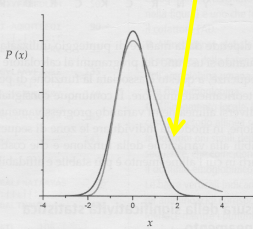
\includegraphics[width=0.5\textwidth]{figures/E.png}\\
\end{center}
In pratica:
\begin{itemize}
    \item allineamo localmente due seq
    \item otteniamo il punteggio $x$
    \item calcoliamo $p(S \geq x)$, la probabilità di
    ottenere un punteggio maggiore di $x$
    nell'ipotesi: le due seq NON sono
    omologhe
    \item se $p < $ soglia (es. 0.01 = 1\%) siamo
    confidenti che siano omologhe.
    \item SEMPRE: serve significatività
    BIOLOGICA oltre che statistica
\end{itemize}
\section{Matrici di punteggio}
Abbiamo già visto che per dare un punteggio a un allineamento
dobbiamo misurare la similitudine fra aa.
Usiamo perciò matrici di punteggio o di sostituzione: saranno
matrici $20x20$. Sono matrici simmetriche: $A \rightarrow B = B \rightarrow A$ (non
sappiamo evolutivamente chi si è trasformato dei due).
\paragraph{Come quantificare la somiglianza degli amminoacidi}
Difficile stabilire criteri oggettivi per le somiglianze fisico-chimiche
degli amino acidi. Non è possibile sapere a priori quali delle varie
caratteristiche fisico-chimiche sono più importanti per le proteine.\\
Emile Zuckerkandl e Linus Pauling (1965) considerarono
frequenze di sostituzione in 18 globine (mioglobine e
emoglobine da uomo a lampreda).
\begin{itemize}
    \item Nero: identità
    \item Grigio: sostituzione molto conservativa (occorrenza$>40\%$)
    \item Bianco: sostituzione abbastanza conservativa (occorrenza $> 21 \%$)
    \item Rosso: non è possibilte osservare sostituzioni
\end{itemize}
\begin{center}
    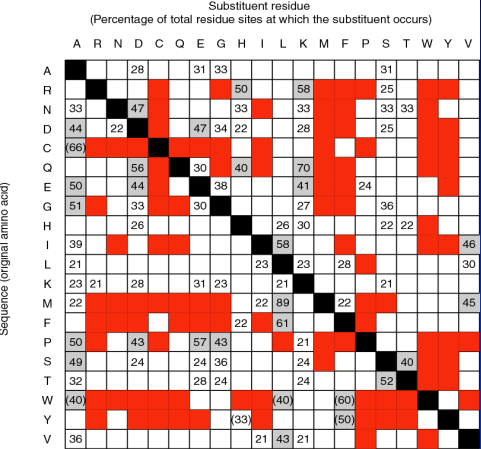
\includegraphics[width=0.5\textwidth]{figures/matx.png}\\
\end{center}
\paragraph{Cosa vogliamo ottenere?} una matrice (PAM250) di score.
Matrice di calcolo che assegna i
punteggi e tollera le discordanze.
Inoltre \dots tutta una serie di matrici di
punteggio, (fino a PAM10) che
è via via meno tollerante con i
disallineamenti.
\subsection{PAM: Point Accepted Mutation}
Mutazione puntuale accettata.
\begin{itemize}
    \item È l'evento in cui il DNA subisce una mutazione che produce il
    cambiamento di un aminoacido
    \item Tale mutazione diviene prevalente in una specie
\end{itemize}
Dayhoff ha osservato famiglie di sequenze identiche all'85\%
(omologhe e molto simili). Le ha allineate e ha creato alberi di
sequenze in cui ha dedotto le sequenze dei progenitori.
Piccoli passi evolutivi, per osservare l'evoluzione e dedurne le
caratteristiche.\\
Le matrici PAM sono basate su allineamenti globali di
proteine strettamente correlate. Il PAM1 è la matrice calcolata dal confronto di sequenze con
non più di 1\% di divergenza. Ad un intervallo evolutivo di
PAM1, un cambiamento si è verificato su una lunghezza di
100 aminoacidi.\\
Altre matrici PAM sono estrapolate da PAM1 ( PAM1 non ha
utilità pratica ). Per PAM250, 250 sostituzioni si sono verificate
tra due proteine su una lunghezza di 100 aminoacidi, nel
passo evolutivo che essa rappresenta.\\
\textit{Nota bene:}Tutti i dati PAM provengono da proteine
strettamente correlate ($>$ 85\% di identità degli aminoacidi).
\newpage
\paragraph{Dayhoff: 34 superfamiglie di proteine}
\begin{center}
    \begin{tabular}{c|c}
        \toprule
        \textbf{Proteina} & \textbf{PAMs per 100 milioni di anni}\\
        \midrule
        Ig kappa chain & 37 \\
        Kappa casein & 33 \\
        luteinizing hormone b & 30 \\
        lactalbumin & 27 \\
        complement component 3 & 27 \\
        epidermal growth factor & 26\\
        proopiomelanocortin & 21\\
        pancreatic ribonuclease & 21 \\
        haptoglobin alpha & 20 \\
        serum albumin & 19 \\
        phospholipase A2, group IB & 19 \\
        prolactin & 17 \\
        carbonic anhydrase C & 16 \\
        Hemoglobin $\alpha$ & 12\\
        Hemoglobin $\beta$ & 12 \\
        apolipoprotein A-II & 10\\
        lysozyme & 9.8 \\
        gastrin & 9.8 \\
        myoglobin & 8.9 \\
        nerve growth factor & 8.5 \\
        myelin basic protein & 7.4 \\
        thyroid stimulating hormone b & 7.4 \\
        parathyroid hormone & 7.3 \\
        parvalbumin & 7.0 \\
        trypsin & 5.9 \\
        insulin & 4.4 \\
        calcitonin & 4.3 \\
        arginine vasopressin & 3.6 \\
        adenylate kinase & 3.2 \\
        triosephosphate isomerase 1 & 2.8 \\
        vasoactive intestinal peptide & 2.6 \\
        glyceraldehyde phosph. dehydrogease & 2.2 \\
        cytochrome c & 2.2 \\
        collagen & 1.7 \\
        troponin C, skeletal muscle & 1.5 \\
        alpha crystallin B chain & 1.5 \\
        glucagon & 1.2 \\
        glutamate dehydrogenase & 0.9 \\
        histone H2B, member Q & 0.9 \\
        ubiquitin & 0
    \end{tabular}
\end{center}
\begin{center}
    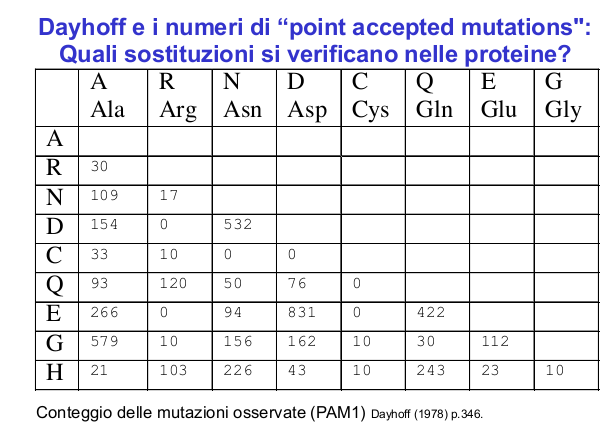
\includegraphics[width=0.5\textwidth]{figures/dayhoff2.png}\\
\end{center}
\subsection{La mutabilità relativa degli amminoacidi}
\paragraph{Quanto spesso mutano nelle proteine?}
Definiamo la Frequenza relativa di mutazione.
\begin{center}
    \begin{tabular}{c | c !{\vline width 2pt} c | c }
        \toprule
        \textbf{AA} & \textbf{Freq} & \textbf{AA} & \textbf{Freq}\\
        \midrule
        Asn & 134 & His & 66 \\
        Ser & 120 & Arg & 65 \\
        Asp & 106 & Lys & 56 \\
        Glu & 102 & Pro & 56 \\
        Ala & 100 & Gly & 49 \\
        Thr & 97 & Phe & 41 \\
        Ile & 96 & Phe & 41 \\
        Gln & 93 & Cys & 20 \\
        Val & 74 & Trp & 18 
    \end{tabular}
\end{center}
\paragraph{Frequenze normalizzate}
\begin{center}
    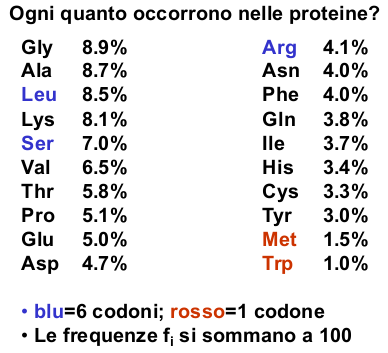
\includegraphics[width=0.5\textwidth]{figures/norm.png}\\
\end{center}
\paragraph{Esempio}
Prendiamo un allineamento multiplo di sequenze,
ad esempio della deidrogenasi gliceraldeide 3-fosfato.\\
\textbf{OSSERVAZIONE:}
le colonne di residui possono avere conservazione alta o bassa.
\begin{center}
    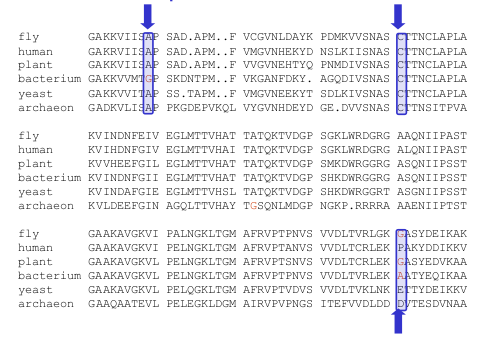
\includegraphics[width=0.5\textwidth]{figures/es3.png}\\
\end{center}
\subsubsection{Matrice PAM1 (probabilità) di Dayhoff}
\begin{center}
    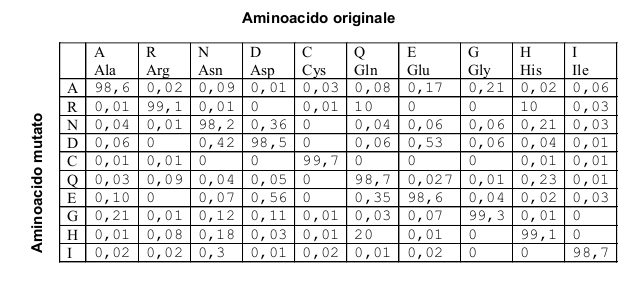
\includegraphics[width=0.5\textwidth]{figures/pam1.png}\\
\end{center}
Ogni elemento della matrice mostra la probabilità che un
amminoacido (in alto) venga sostituito da un altro aminoacido
(a lato).
\section{Matrici di sostituzione}
Una matrice di sostituzione contiene valori proporzionali
alla probabilità che l'amminoacido i muti nell' amminoacido $j$
per tutte le coppie possibili di aminoacidi. Le matrici di sostituzione sono costruite assemblando
un campione ampio e diversificato di allineamenti a coppie
(o allineamenti multipli di sequenza) di aminoacidi.\\
Le matrici di sostituzione dovrebbero riflettere la probabilità
reale di mutazione in un periodo di evoluzione.
I due principali tipi di matrici di sostituzione: PAM e BLOSUM.
\subsection{Moltiplicare le matrici}
Con (PAM1)$^\wedge$n si può simulare il passaggio di n passi di
evoluzione.
\begin{center}
    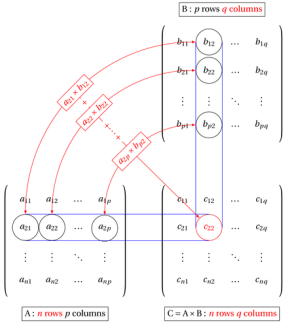
\includegraphics[width=0.5\textwidth]{figures/pamn.png}\\
\end{center}
\paragraph{Matrice di sostituzione PAM0 (probabilità)} Ovvero: nulla cambia.
\begin{center}
    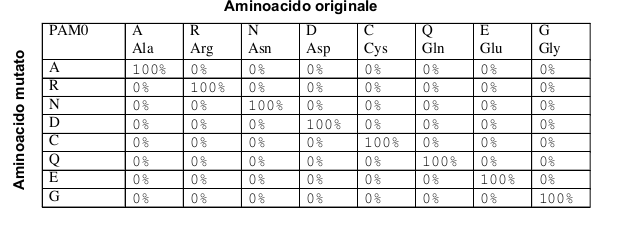
\includegraphics[width=0.5\textwidth]{figures/pam0.png}\\
\end{center}
Si sono verificati 0 passi di evoluzione: non è cambiato nulla!
\paragraph{Matrice di sostituzione PAM2000 (probabilità)} PAM1$^\wedge$2000, ovvero: il caso.
\begin{center}
    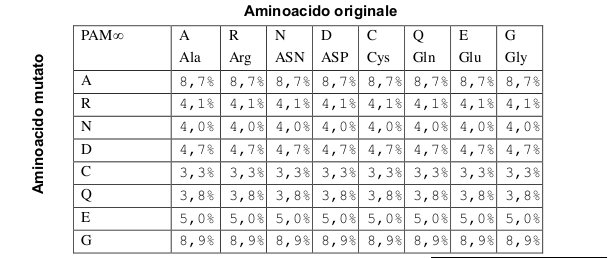
\includegraphics[width=0.5\textwidth]{figures/pam2000.png}\\
\end{center}
Moltiplicando PAM1 per 2000 (passi di
evoluzione)si arriva ad una situazione in cui la
probabilità converge alla frequenza osservata
\paragraph{Matrice di sostituzione PAM250 (probabilità) di mutazione} 
\begin{center}
    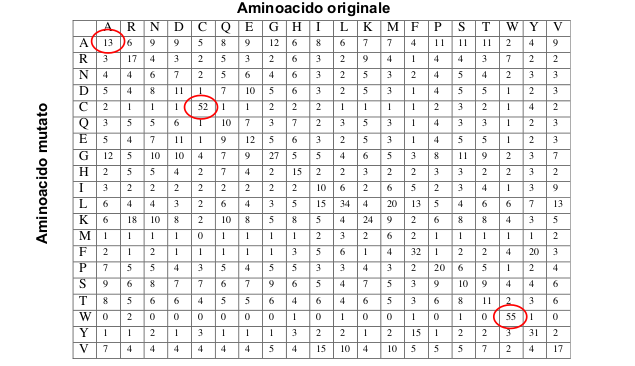
\includegraphics[width=0.5\textwidth]{figures/pam250.png}\\
\end{center}
PAM 250 è un caso interessante: ottenuta da PAM1$^\wedge$250 prevede che circa il 20\%
della sequenza sia conservato. A $ \rightarrow$ A ha probabilità del 13\%. Da notare W e C che
anche dopo 250 mutazioni hanno il 50\% di probabilità di non mutare.
\subsection{Approccio Dayhoff}
\paragraph{per l'assegnazione di punteggi per ogni due residui di aminoacidi allineati}
Dayhoff et al. hanno definito il punteggio (score) per due generici
residui $i,j$:
\begin{itemize}
    \item $q_{i,j} = $ probabilità che l'aminoacido $i$ venga sostituito da $j$\\(probabilità di omologia in base alle sostituzioni osservate)
    \item $p_{i,j} = $ Probabilità di trovare casualmente l'appaiamento $i,j$\\(prodotto della probabilità di trovare un “$i$” e quella di trovare un “$j$” in una
    qualunque sequenza, cioè prodotto delle frequenze)
\end{itemize}
Il loro rapporto serve a tenere conto che l'evento $q_{i,j}$
sia casuale.\\
Il valore è poi convertito al log (per rendere due valori sommabili) e moltiplicato
per 10 (così che, prendendo la parte intera del valore si conserva la prima cifra
decimale). Gli score sono utili negli allineamenti a coppie (e in algoritmi di
ricerca come BLAST)
$$ s_{i,j} = 10 \times log({q_{i,j}\over p_{i,j}})$$
$S(trp,trp) = 10 Log({0.55\over 0.010}) = 17,4$ significa che la probabilità di trovare un
$W$ conservato è 50 volte maggiore della
probabilità che un $W$ sia a caso nelle due
posizioni considerate.\\
Un -10 è un $-1(log)$ quindi ${1\over 10}$ e indica che la probabilità che quell'allineamento si verifichi è ${1\over 10}$ della frequenza di quegli amminoacidi in posizioni corrispondenti.
\paragraph{Matrici PAM a confronto}
\begin{center}
    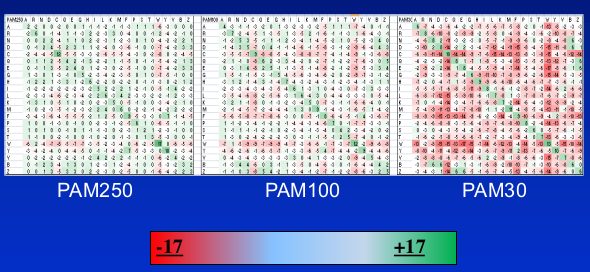
\includegraphics[width=0.5\textwidth]{figures/pamconf.png}
\end{center}
\newpage
\begin{center}
    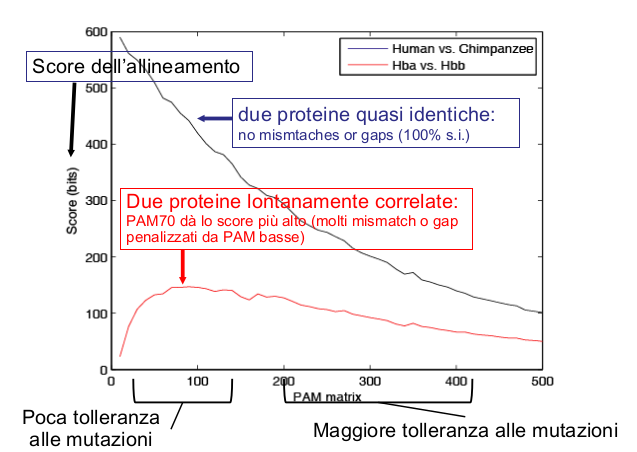
\includegraphics[width=1.25\textwidth]{figures/prot.png}
\end{center}
\newpage
\section{Matrici BLOSUM}
Le matrici BLOSUM sono basate su allineamenti locali, tratti
dal database BLOCKS che raggruppa blocchi (regioni) di
allineamenti locali di sequenze lontanamente correlate. BLOSUM sta per BLOck SUbstitution Matrix.\\
BLOSUM62 è una matrice calcolata a partire da sequenze
con divergenza minore del 62\%. Default per BLAST .
Il metodo di calcolo degli score è poi simile a quello per le
PAM, ma si usa $\lambda = 2$ al posto di 10 (infatti per BLOSUM il range è $90-45$ VS $30-250$ per le PAM)
$$ S_{i,j} = ({1\over \lambda}) log ({p_{i,j}\over q_i * q_j})$$
\begin{center}
    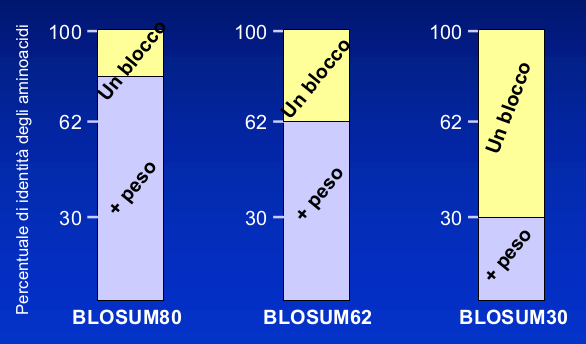
\includegraphics[width=0.7\textwidth]{figures/blosum.png}
\end{center}
\begin{center}
    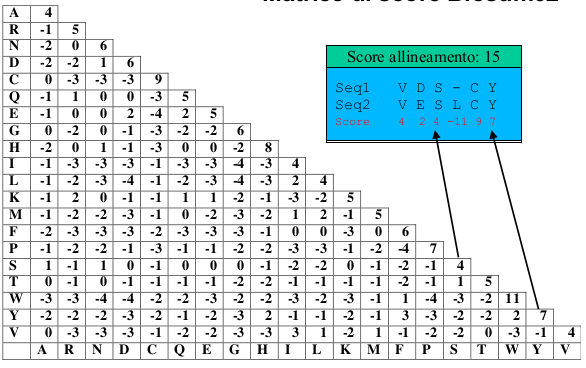
\includegraphics[width=0.7\textwidth]{figures/scorblosum.png}\\
    \Large
    Punteggio$_{totale} = \sum $ somiglianze $- \sum$ penalità gap
\end{center}
\section{BLOSUM vs. PAM}
PAM si basa su principi evoluzionistici, mentre BLOSUM si basa
più sull'osservazione di allineamenti reali, senza fare assunzioni di
omologia.
\begin{center}
    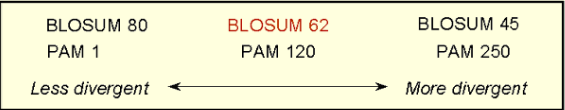
\includegraphics[width=0.7\textwidth]{figures/vs.png}
\end{center}

\begin{minipage}[t]{.4\textwidth}
    \raggedright
    \textbf{Più conservativo}\\
    \underline{es.Globina: topo vs ratto}\\
    Nella BLOSUM 80 le sequenze
    identiche per l'80\% finiscono in un
    unico blocco e gli score sono
    applicati considerando gli altri
    allineamenti $\rightarrow$ score adatti per
    proteine simili (come per la PAM10)
    \end{minipage}%
    \begin{minipage}[t]{.5\textwidth}
        \raggedleft
        \textbf{Meno conservativo}\\
        \underline{es.Globina: topo vs batterio}\\
        Nella BLOSUM 45 le sequenze
        identiche per il 45\% finiscono un unico
        blocco e gli score sono applicati
        considerando gli altri allineamenti $\rightarrow$
        score adatti per proteine diverse
        (come per la PAM250)
    \end{minipage}
\subsection{La "Twilight zone" nell'allineamento di proteine}
\paragraph{Quando compariamo due sequenze proteiche simili,
quante mutazioni possono accumularsi prima che le
differenze le rendano irriconoscibili?}
L'identità tra due sequenze ciascuna di 100 aminoacidi cala
come un esponenziale negativo all'accumularsi delle
mutazioni.\\
\begin{itemize}
    \item A PAM1, due proteine sono al 99\% identiche
    \item A PAM10.7, ci sono 10 differenze ogni 100 residui
    \item A PAM80, ci sono 50 differenze ogni 100 residui
    \item A PAM250, ci sono 80 differenze ogni 100 residui
\end{itemize}
Oltre (20-25\% identità) non è più distinguibile una
similitudine (Allineamenti multipli, modeling)
\begin{center}
    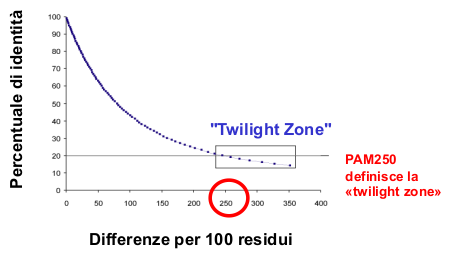
\includegraphics[width=0.5\textwidth]{figures/twilight.png}
\end{center}

\begin{titlepage}
    \begin{center}
        \vspace*{1cm}
        \LARGE
        \textbf{Lezione 5: BLAST\\Basic Local Alignment Search Tool}

    \end{center}
\end{titlepage}
\setcounter{page}{45}

\section{BLAST}
\subsection{Problema con gli algoritmi dinamici}
Gli algoritmi visti (WS, NW) sono precisi ma lenti.
Servono metodi euristici: trovano soluzioni
approssimate ma vicine a quella ottimale in tempi
brevi.\\
Spesso la domanda è: \textit{data una sequenza query, quali
sequenze simili sono note e già presenti nei
databases?}\\
Tra i metodi euristici più usati per la ricerca di singole
sequenze in banche dati troviamo FASTA e BLAST.
\subsection{Cos'è Blast?}
BLAST (Basic Local Alignment Search Tool)
permette un confronto rapido tra una sequenza
query e il contenuto di un database.
L'algoritmo di BLAST è:
\begin{itemize}
    \item veloce
    \item accurato
    \item web-accessibile 
\end{itemize}
BLAST è fondamentale per capire la relazione di
una sequenza query con altre proteine o
sequenze di DNA note.\\
I suoi utilizzi comprendono:
\begin{itemize}
    \item individuare ortologhi e paraloghi
    \item scoperta di nuovi geni o proteine
    \item scoperta di varianti di geni o proteine noti
    \item lo studio delle expressed sequence tags (EST)
    \item lo studio di struttura e funzione delle proteine
\end{itemize}
\subsection{Ricerca su blast}
Le quattro fasi di una ricerca BLAST:
\begin{enumerate}
    \item Scegliere la sequenza (query)
    \item Selezionare il tipo di programma BLAST
    \item Selezionare il database per la ricerca
    \item Scegliere i parametri opzionali
    \item Quindi fare clic su "BLAST"
\end{enumerate}
\begin{center}
    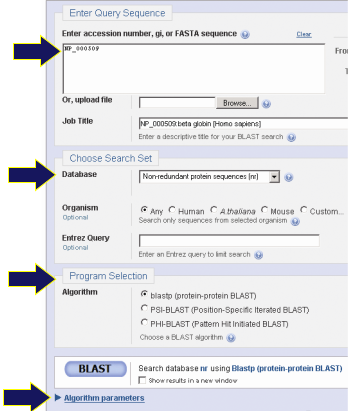
\includegraphics[width=0.3\textwidth]{figures/blast.png}
\end{center}
\paragraph{Passo 1: Scelta della sequenza}
La sequenza può essere inserita in
formato FASTA o come accession
number (RefSeq).\\Esempio:
\begin{center}
    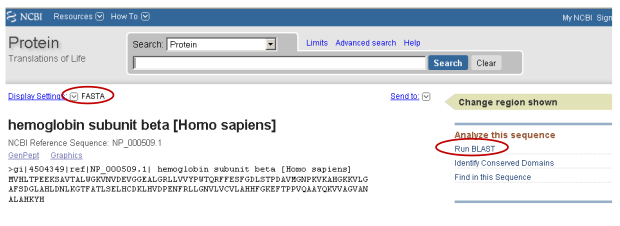
\includegraphics[width=0.5\textwidth]{figures/blast1.png}
\end{center}
\paragraph{Passo 2: Scegli il programma BLAST}
\begin{itemize}
    \item blastn (nucleotide BLAST)
    \item blastp (protein BLAST)
    \item blastx (BLAST tradotto n $\rightarrow$ P)
    \item tblastn (BLAST tradotto p $\rightarrow$ N)
\end{itemize}
Ci sono anche altri tools disponibili.
\begin{center}
    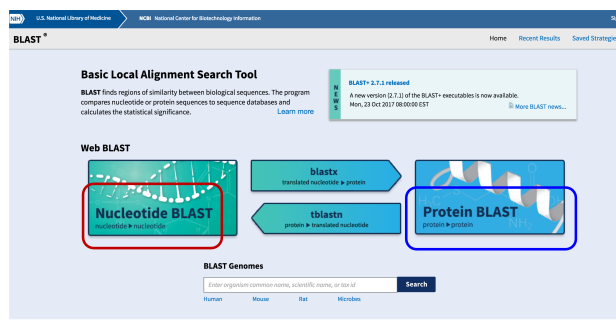
\includegraphics[width=0.5\textwidth]{figures/blast2.png}
\end{center}
\paragraph{Passo 3: scegliere il database}
\begin{itemize}
    \item \textbf{nr} 
        \subitem Non ridondante (database più generale,
        ritorna una sequenza e diversi riferimenti
        in database in cui la stessa è presente)
    \item \textbf{refseq}
        \subitem Solo sequenze con codice refse q
    \item \textbf{dbest} 
        \subitem Database di EST
    \item \textbf{dbsts}
        \subitem Database di sequenze localizzate
    \item \textbf{gss}
        \subitem Genome sequence surveys ( BAC, Yac, ecc )
    \item \textbf{altri}
        \subitem Pdb, genomi completi, solo sequenze oggetto
        di brevetti (pat), \dots
\end{itemize}
\paragraph{Fase 4: parametri opzionali}
Si può:
\begin{itemize}
    \item Scegliere l'organismo di ricerca
    \item Attivare filtri
    \item Modificare la matrice di punteggio
    \item Cambiare il valore minimo di affidabilità dei risultati
    \item Modificare la dimensione della parola W
\end{itemize}
Allo stesso modo in blastp e blastn:
\begin{center}
    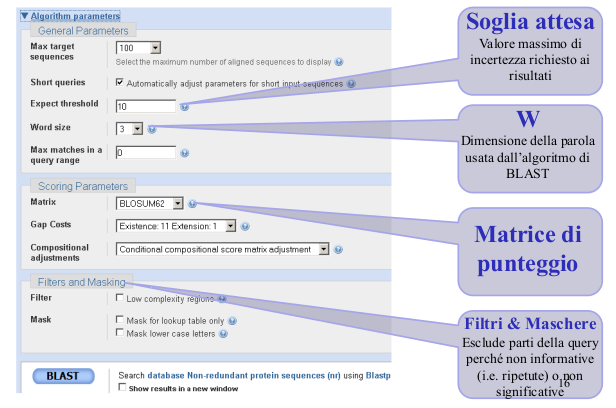
\includegraphics[width=0.5\textwidth]{figures/fase4.png}
\end{center}
\paragraph{L'output}
\begin{center}
    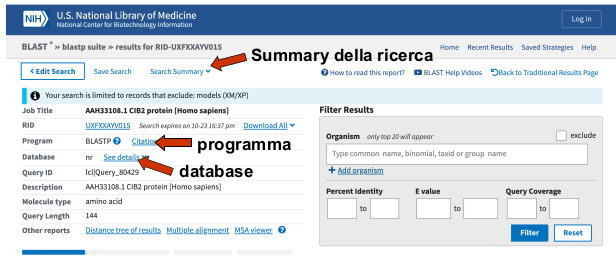
\includegraphics[width=0.5\textwidth]{figures/output.png}
\end{center}
\subsection{L'algoritmo}
\paragraph{BLAST: le basi dell'allineamento di sequenze}
L'allineamento può essere:
\begin{enumerate}
    \item \textbf{Globale}\\
    (Needleman \& Wunsch)
    \subitem Usa la programmazione dinamica per trovare i migliori
    allineamenti tra due sequenze.
    (Anche se gli allineamenti sono ottimali, la ricerca non è
    esaustiva). I gap sono ammessi e l'intera lunghezza delle
    sequenze è allineata (da cui "globale").
    \item \textbf{Locale}\\
    (Smith \& Waterman, 1980 -  modifica del primo (per all. globale))
    \subitem L'allineamento può riguardare solo una parte di una delle
    sequenze, ed è adatto alla ricerca di caratteristiche locali
    comuni alle sequenze (domini, siti attivi, ecc).
\end{enumerate}
BLAST è una approssimazione euristica per l'allineamento
locale. Esamina solo una parte dello spazio di ricerca.
\paragraph{Come funziona una ricerca BLAST?}
\epigraph{L'idea centrale dell'algoritmo di BLAST è di
limitare l'attenzione a coppie di segmenti in cui
si allineano parole di lunghezza w con un
punteggio di almeno T.}{\textit{Altschul et al. (1990)}}
\subsubsection{Le 3 fasi}
\paragraph{Fase 1}compilare una lista di coppie di parole (di
lunghezza $w = 3$) con un punteggio oltre la soglia $T$.
\begin{center}
    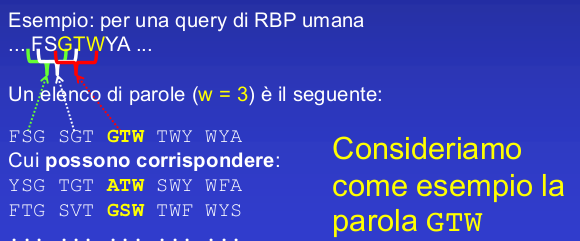
\includegraphics[width=0.5\textwidth]{figures/fas1.png}
\end{center}
Se pongo la soglia $T = 11$, gli allineamenti con punteggio maggiore della soglia sono:
\begin{itemize}
    \item GTW $6+5+11 \rightarrow 22$
    \item GSW $6+1+11 \rightarrow 18$
    \item ATW $0+5+11 \rightarrow 16$
    \item NTW $0+5+11 \rightarrow 16$
    \item GTY $6+5+2 \rightarrow 13$
\end{itemize}
Gli allineamenti con punteggio minore della soglia:
\begin{itemize}
    \item GNW $\rightarrow 10$
    \item GAW $\rightarrow 9$
\end{itemize}
Dunque saranno esclusi dai passi successivi.
\paragraph{Fase 2}Scansione del database per le voci che
corrispondono alla lista compilata (con punteggio
maggiore della soglia $T$). È un passo veloce e relativamente semplice: i
database sono indicizzati per la ricerca di parole di
lunghezza $W$.
\paragraph{Fase 3}Quando si riesce a trovare una corrispondenza Fase 3 : nella versione originale di BLAST (1990)
(abbinamento tra una “parola” con punteggio maggiore $T$ al database),
estendere l'allineamento in entrambe le direzioni.
\begin{itemize}
    \item Tenere traccia del punteggio (utilizzando la matrice di
    punteggio)
    \item Stop quando il punteggio è inferiore a una certa soglia.
\end{itemize}
\begin{center}
    \includegraphics[width=0.5\textwidth]{figures/fase3.png}
\end{center}
Nella versione originale di BLAST (1990) ciascun hit è esteso in entrambe le direzioni.\\
Nella versione migliorata, dal 1997, sono necessari due
hit vicini (entro una distanza A). In questo modo le
estensioni avvengono meno frequentemente ma si
ottiene un notevole risparmio di tempo
\paragraph{I parametri}
È possibile personalizzare i parametri di BLAST, sia per le soglie
menzionate che per le dimensioni delle parole w (default 3 per le
proteine, 6 negli algoritmi più recenti, e 11 per le sequenze
nucleotidiche).
E 'importante valutare la significatività statistica dei risultati
della ricerca.
Ecco che effetto ha la scelta di diversi valori della soglia $T$.
Parole più grandi
producono meno
hits, velocizzando
la ricerca, a scapito
della sensibilità.
\begin{center}
    \includegraphics[width=0.5\textwidth]{figures/param.png}
\end{center}
\subsection{Come interpretare una ricerca BLAST}
È importante valutare la significatività statistica dei risultati
della ricerca. Per gli allineamenti globali, gli aspetti statistici non sono
molto approfonditi.\\
Per gli allineamenti locali (compresi i risultati di ricerca
BLAST), le statistiche sono più solide. I punteggi seguono
una distribuzione del valore estremo (EVD), piuttosto che
una distribuzione normale.
La densità di probabilità del valore estremo
($u$ valore caratteristico = 0 e costante di decadimento $\lambda$ = 1)
È spostata a destra rispetto alla distribuzione normale.
\begin{center}
    \includegraphics[width=0.5\textwidth]{figures/dist.png}
\end{center}
\subsubsection{Il valore atteeso E}
È il numero di allineamenti (high scoring segment pairs o HSP)
con punteggio maggiore o uguale a un punteggio $S$ che
dovrebbero verificarsi per caso in quella ricerca sul database.
Si può pensarlo come un indice di incertezza.
Un valore $E$ è correlato a un valore di probabilità $p$.\\
L'equazione fondamentale che descrive un valore $E$ è: 
$$ E = KMN e^{\lambda S}$$
Con:
\begin{itemize}
    \item $M$, lunghezza della query
    \item $N$, lunghezza della sequenza nel database
    \item $S$, score
    \item $K, \lambda$, parametri che dipendono dallo scoring system ($\lambda$) dal database usato ($K$)
\end{itemize}
\paragraph{Alcune proprietà}
\begin{itemize}
    \item Il valore di $E$ decresce esponenzialmente con l'aumentare $S$.
    Valori più elevati di $S$ corrispondono a migliori allineamenti e
    infatti hanno $E$ values più bassi.
    \item Ottenere un allineamento con $E = 1$ significa che esiste un
    altro allineamento con lo stesso score $S$ che è risultato per
    caso.
    \item La stessa ricerca, su un database più piccolo o più grande,
    anche se restituisce lo stesso allineamento deve avere un
    valore di $E$ diverso (ciò dipende da $K$).
\end{itemize}
\paragraph{Punteggio, dallo score grezzo (S) in bit}
Ci sono due tipi di punteggi:
\begin{itemize}
    \item punteggi grezzi (calcolato da una particolare matrice di
    sostituzione)
    \item punteggi bit (punteggio normalizzato)
\end{itemize}
I punteggi in bit sono paragonabili tra diverse ricerche
(es. diverse matrici di sostituzione o diverse banche dati)
perché sono normalizzati, adatti quindi al paragone anche se
originati tramite diverse matrici di punteggio e database di
dimensione diversa
$$ S' = bitScore = {(\lambda S - ln(K))\over ln(2)} $$
\subsubsection{E-value e p-value}
Il valore atteso $E$ è il numero di allineamenti con punteggio
maggiore o uguale a un punteggio $S$ che dovrebbero verificarsi
per caso in un database di ricerca.\\
Il \textit{p-value} è un modo diverso (ma equivalente) di rappresentare
la significatività di un risultato.
$$ p = 1 -e^{-E}$$
Per valori molto piccoli E e p sono molto simili. Tuttavia tra 1 e
10 il valore di E è più chiaro (poichè riflette un numero di hits).
\begin{center}
    \begin{tabular}{c|c}
        E & p \\
        \midrule
        10 & 0.99995460\\
        5 & 0.99326205\\
        2 & 0.86466472\\
        1 & 0.63212056\\
        0.1 & 0.09516258 (circa 0.1)\\
        0.05 & 0.04877058 (circa 0.05)\\
        0.001 & 0.00099950 (circa 0.001)\\
        0.0001 & 0.0001000\\
    \end{tabular}
\end{center}
\subsubsection{Panoramica}
\begin{itemize}
    \item \textbf{W:} Dimensione della parola usata dall'algoritmo di Blast
    \item \textbf{Soglia attesa:} Valore massimo di incertezza richiesto ai risultati
    \item \textbf{Costo gap:} Apertura ed estensione
    \item \textbf{Matrice di punteggio}
    \item \textbf{Soglia T di punteggio}
    \item \textbf{Dimensione del database}
    \item \textbf{Parametri per il calcolo di E}
\end{itemize}
\paragraph{In quali casi ha senso una soglia E elevata?}
Si supponga di eseguire una ricerca con una query corta
(ad esempio 9 aminoacidi). Non ci sono residui sufficienti per
accumulare un punteggio elevato (o un valore di E piccolo).
Infatti, una corrispondenza di tutti e 9 i residui potrebbe
produrre un punteggio basso con un valore di E =100 o 200.
E tuttavia, questo risultato potrebbe essere "reale" e di vostro
interesse.
In casi particolari, impostando il valore di cut-off per E a
20.000 non si cambia il modo in cui è stata fatta la ricerca,
ma cambiano i risultati riportati.
\subsection{Strategia per la ricerca con BLAST}
\begin{itemize}
    \item Concetti generali
    \item Come valutare la significatività dei risultati
    \item Come gestire troppi risultati
    \item Come gestire troppo pochi risultati
    \item Blast e la valutazione dell'omologia
\end{itemize}
\paragraph{A volte un vero match ha un valore di E > 1}
\begin{center}
    \includegraphics[width=0.5\textwidth]{figures/realmatch.png}
\end{center}
Posso provare un BLAST reciproco per confermare.\\
A volte un valore E simile si verifica sia per un match esatto corto che per uno lungo.
\begin{center}
    \includegraphics[width=0.5\textwidth]{figures/match.png}
\end{center}
I risultati delle ricerche, ordinati per E, si valutano poi nel dettaglio!
\subsubsection{Valutare se le proteine sono omologhe}
\textit{Es.lipocaline: hanno bassa s.i. ma struttura 3D simile}\\
\paragraph{RBP4 (query) e Salivary Lipocalin from boar:} Basso punteggio bit, valore E=0.40, il 21% di identità
(“twilight zone"). Ma sono davvero omologhe. Prova un'altra
ricerca BLAST con la seconda come query, per trovare
molte altre lipocaline.\\
L'universo di lipocaline (proteine che trasportano piccoli ligandi idrofobici).
\begin{center}
    \includegraphics[width=0.5\textwidth]{figures/lipocaline.png}
\end{center}
\begin{enumerate}
    \item La ricerca con BLAST con salivary lipocalin [Sus
    scrofa] come query trova molte altre lipocaline
    \item Utilizzando la beta globina umana come una query, ecco i risultati
    blastp contro le proteine umane RefSeq (PAM30). Dove si trova
    mioglobina? È assente!
    \item Abbiamo bisogno di usare PSI-BLAST
\end{enumerate}
\subsubsection{Due esempi di problemi che BLAST standard non può risolvere}
\begin{enumerate}
    \item Usando la beta globina umana come query
    contro proteine umane con RefSeq, blastp non
    “trova“ la mioglobina umana. Questo perché le due
    proteine sono troppo distanti. PSI-BLAST presso
    NCBI così come i modelli nascosti di Markov
    possono facilmente risolvere questo problema.
    \item Come possiamo cercare con 10000 paia o addirittura milioni di paia di basi come query?\\Molti strumenti tipo-BLAST per il DNA genomico sono
    disponibili come PatternHunter, Megablast, Blat, e
    BLASTZ (NON li vedremo nel corso).
\end{enumerate}
\section{PSI-BLAST (position specific iterated)}
Lo scopo di PSI-BLAST è quello di cercare
più in profondità nel database match alla
sequenza della proteina query, utilizzando
una matrice di punteggio che è adattata
dinamicamente (in modo iterativo) per la
ricerca in corso.
\subsection{Fasi di esecuzione}
\begin{enumerate}
    \item Selezionare una query di ricerca (diverse sequenze) contro
    un database proteico e lanciare BLASTP
    \item PSI-BLAST costruisce un allineamento multiplo di sequenze
    a partire dagli hit migliori e crea quindi un "profilo" detto anche
    Matrice di calcolo posizione-specifica (PSSM, position-
    specific scoring matrix)
    \item Il PSSM (e non più la sequenza iniziale) è usato come query
    sul database: mi aspetto ora di trovare più sequenze sui cui
    ricalcolare l'allineamento multiplo
    \item PSI-BLAST stima la significatività statistica (valori di E)
    \item Ripetere i passaggi 3 e 4 in modo iterativo, tipicamente 5
    volte. Ad ogni nuova ricerca, un nuovo profilo viene utilizzato nella
    query.
\end{enumerate}
Un PROFILO di lunghezza L è una matrice L X 20 (per
proteine, o L X 4 per DNA) di elementi s i,j rappresentanti lo
score per allineare la lettera j alla posizione i.
Un profilo può essere allineato ad una sequenza individuale
esattamente allo stesso modo di una normale sequenza
\subsubsection{Come costruire il profilo?} Esaminare l'output di blastp per identificare "regole”
empiriche di punteggio per gli aminoacidi tollerati in ogni
posizione: non tutte le posizioni ammettono la stessa
variabilità. Il punteggio ne terrà conto.
\subsubsection{Funzionamento di Psi-Blast}
\begin{center}
    \includegraphics[width=0.8\textwidth]{figures/psiblast.png}
\end{center}
\begin{itemize}
    \item In riga: 20 amminoacidi
    \item In colonna: tutti gli aa della posizione 1 alla fine (L) della proteina query per PSI-BLAST
    \item Notare che dato un amminoacido (come ad esempio l'alanina) nella sequenza query, si possono ottenere diversi punteggi per il match, in relazione alla posizione nella sequenza query e alla frequenza in cui la ritrovo nell'allineamento multiplo.
    \item Lo stesso vale anche per il triptofano: posizioni diverse hanno, per lo stesso match, punteggi diversi
\end{itemize}
\paragraph{In pratica:} il profilo posizione-specifico (PSSM) cattura il
pattern di conservazione nell'allineamento multiplo ottenuto
dai migliori hits di BLASTP e lo immagazzina sottoforma di
matrice di score $\rightarrow$ Posizioni altamente conservate ottengono punteggi alti;
posizioni poco conservate ottengono punteggi bassi.\\
Il profilo è quindi una specie di nuova query in cui ogni
posizione ha un “peso” differenziato: questa informazione
può essere utilizzata per estendere la ricerca.
\subsubsection{Esempio di Cicli}
Schematicamente, questi gli step per i primi due cicli:
\begin{itemize}
    \item CICLO 1: singola query, 1 run di BLAST\\\includegraphics[width=0.4\textwidth]{figures/ciclo1.png}
    \item CICLO 2: PSSM come query, più sequenze trovate\\\includegraphics[width=0.4\textwidth]{figures/ciclo2.png}
\end{itemize}
\begin{center}
    \begin{tabular}{ccc}
        \toprule
        \textbf{Iterazioni} & \textbf{\#Hits} & \textbf{\#Hits > Soglia}\\
        \midrule
        1 & 104 & 49\\
        2 & 173 & 96\\
        3 & 236 & 178\\
        4 & 301 & 240\\
        5 & 344 & 283\\
        6 & 342 & 298\\
        7 & 378 & 310\\
        8 & 382 & 320
    \end{tabular}
\end{center}
Nota: (come prima, globina beta, PAM30, RefSeq, Homo
sapiens). Gli E-values cambiano a seconda delle
interazioni, e possono migliorare drasticamente. Seguiamo iterativamente l'allineamento con la subunità mu.
\begin{itemize}
    \item Iterazione 1:\\
    \begin{center}
        \includegraphics[width=0.8\textwidth]{figures/it1.png}
    \end{center}
    \item Iterazione 2:\\
    \begin{center}
        \includegraphics[width=0.8\textwidth]{figures/it2.png}
    \end{center}
    \item Iterazione 3:\\
    \begin{center}
        \includegraphics[width=0.8\textwidth]{figures/it3.png}
    \end{center}
    \item Iterazione 4:\\
    \begin{center}
        \includegraphics[width=0.8\textwidth]{figures/it4.png}
    \end{center}
    \item Iterazione 5:\\
    \begin{center}
        \includegraphics[width=0.8\textwidth]{figures/it4.png}
    \end{center}
    \item E non migliora più (e nemmeno il bit-score)
\end{itemize}
Le matrici di score permettono di campionare una regione
relativamente limitata dell'universo delle sequenze:
\begin{center}
    \includegraphics[width=0.8\textwidth]{figures/mat.png}
\end{center}
PSI-BLAST genera matrici di punteggio più potenti delle PAM o BLOSUM
\subsection{Psi-Blast: la corruzione}
PSI-BLAST è utile per rilevare relazioni deboli ma
biologicamente significative tra le proteine.La principale fonte di falsi positivi è la falsa amplificazione di
sequenze non correlate alla query.\\
\textit{Esempio:} una query con un motif
coiled-coil può rilevare migliaia di
altre proteine con questo motivo che
non sono omologhe.\\
Una volta che anche una singola proteina spuria è inclusa
in una ricerca PSI-BLAST entro la soglia, non ne uscirà e influenzerà la iterazioni successive.\\
La \textbf{corruzione} è definita come la presenza di almeno un
falso allineamento positivo con un valore E <10 -4 dopo
cinque iterazioni.
Tre approcci per arrestare la corruzioni:
\begin{enumerate}
    \item Applicare filtri alle regioni con composizione poco
    specifica
    \item Aggiustare il valore di E da 0.001 (default) ad uno più
    basso, come E = 0.0001.
    \item Controllare visivamente l'output di ogni iterazione.
    Rimuovere gli hit sospetti deselezionando la casella.
\end{enumerate}

\begin{titlepage}
    \begin{center}
        \vspace*{1cm}
        \LARGE
        \textbf{Lezione 6: Allineamenti Multipli di Sequenze}

    \end{center}
\end{titlepage}
\setcounter{page}{59}
\section{Allineamento multiplo di sequenze}
\subsection{Visione Generale}
\subsubsection{Una definizione}
Un allineamento multiplo è una collezione di tre o più sequenze proteiche (o nucleotidiche) parzialmente o completamente allineate
\begin{itemize}
    \item I residui e le zone omologhe sono allineate in colonne per tutta la lunghezza delle sequenze
    \item Il senso dell'omologia dei residui è evoluzionistico
    \item Il senso dell'omologia dei residui è strutturale
\end{itemize}
Si tratta di un argomento di ricerca attivo dagli anni '90.
\subsubsection{Alcuni fatti}
Non c'è necessariamente un allineamento "corretto" per una famiglia di proteine.\\
\textbf{Perchè?}
    \begin{itemize}
        \item Le sequenze di proteine evolvono
        \item Le corrispondenti strutture tridimensionali evolvono, anche se più lentamente
        \item Può essere particolarmente difficile identificare i residui che si sovrappongono nello spazio (strutturalmente) in un allineamento multiplo di sequenze.
    \end{itemize}
Due proteine che condividono il 30\% di identità di sequenza avranno circa il 50\% dei residui sovrapponibili nelle due strutture
\subsubsection{Caratteristiche utili per realizzzarlo}
Alcuni residui allineati, come cisteine che formano ponti disolfuro, o i triptofani, possono essere altamente conservati
    \begin{itemize}
        \item Ci possono essere motivi conservati come un dominio transmembrana
        \item Alcune caratteristiche come le strutture secondarie, siti attivi e di legame per ligandi o complessi sono spesso conservate
        \item Ci possono essere regioni con inserimenti o delezioni propagati in parte della famiglia.
        \item I principi che vedremo sono focalizzati sulle proteine ma sono validi in generale anche per sequenze nucleotidiche.
    \end{itemize}
\subsubsection{Utilizzi e Vantaggi}
    \begin{itemize}
        \item Il MSA è più sensibile di quello a coppie nel rilevamento di omologie, per questo è uno strumento essenziale nella costruzione di modelli strutturali per omologia
        \item L'output di BLAST può assumere la forma di un MSA, e possono essere individuati residui conservati o motivi
        \item In un MSA si possono analizzare i dati di una popolazione
        \item Una singola query può essere cercata contro un database di MSA (ad esempio Pfam)
        \item Le regioni regolatorie dei geni sono spesso identificabili da MSA
    \end{itemize}
\subsection{Metodi Euristici}
I metodi esatti non vengono trattati in questa sede: non ci sono soluzioni efficienti e già con 5 sequenze il tempo di computazione è eccessivo (esponenziale)
\textbf{Metodi progressivi}: usano un albero guida (analogo ad un albero filogenetico) per determinare come combinare uno per uno allineamenti a coppie
(progressivamente) per creare un allineamento multiplo.\\
Esempi: CLUSTAL OMEGA (W), MUSCLE (usato da HomoloGene)
\section{Clustal Omega}
Usa Clusta Omega per fare un MSA progressivo.
\subsection{Fasi di MSA}
\paragraph{Il MSA progressivo di Feng-Doolittle (1987) alla base di Clustal (W) avviene in 3 fasi}
\begin{enumerate}
    \item Realizzare una serie di allineamenti a coppie globali (Needleman e Wunsch, algoritmo di programmazione dinamica) di cui si calcola la distanza (matrice delle distanze)
    \item Creare un albero guida a partire dalla matrice delle distanze
    \item Allineare progressivamente le sequenze
\end{enumerate}
\subsubsection{Feng Doolittle fase 1: generare allineamenti}
\normalsize{Generare allineamenti a coppie globali}\\
\small{Esempio: allineare 5 globine (1, 2, 3, 4, 5).}\\
\paragraph{Primo step: a due a due e valutare gli score di ogni possibile allineamento a coppie\\}
\textbf{Numero di allineamenti a coppie necessari per coprire tutte le possibili combinazioni}
\begin{itemize}
    \item Per n sequenze, (n-1) (n) / 2
    \item Per 5 sequenze, (4) (5) / 2 = 10
    \item Per 200 sequenze, (199) (200) / 2 = 19.900
\end{itemize}…Quindi per molte sequenze ClustalW è molto lento ed è preferibile usare metodi più veloci (MUSCLE è molto veloce).
\subsubsection{Feng-Doolittle fase 2: albero guida}
\textbf{Convertire i punteggi di similitudine in punteggi di distanza:} è matematicamente più semplice, oltre che più intuitivo, lavorare con le distanze. Una semplice definizione di distanza è data dalla percentuale di
residui diversi (100- SI in \%) che viene inserita nella matrice delle distanze.
\begin{itemize}
    \item Dalla matrice delle distanze si calcola l'albero guida con il metodo di clustering neighbor joining che vedrete nel modulo 2.
    \item Vediamo un semplice esempio di clustering e costruzione di albero guida
\end{itemize}
\paragraph{Il clustering alla base di CLUSTAL(W)} È una matrice di distanze, minore è il numero, maggiore è la similitudine.
\textit{Nota: tutte le distanze tra la I e la IV riga sono minori di quelle riportate nella V}
\begin{center}
    \includegraphics[width=0.8\textwidth]{figures/clustal.png}
\end{center}
\begin{itemize}
    \item Tutte le sequenze vengono poi allineate progressivamente, seguendo le indicazioni dell'albero
    guida: prima si allineano le più simili (vicine) e poi progressivamente le più distanti.
    \item A ogni passaggio si utilizza un algoritmo dinamico di allineamento molto efficiente che accoppia sequenze o gruppi di sequenze
    \item Il MA è composto a partire a tanti allineamenti a coppie, anche fra gruppi di sequenze.
    \item[] \textit{Nota: Le indel presenti negli allineamenti già effettuati restano fisse.}
    \item[]\includegraphics[width=0.5\textwidth]{figures/albero1.png}
    \item Come allineare pogressivamente due gruppi di sequenze? Si usa sempre una matrice. È simile all'allineamento dinamico di due sequenze visto.
    \item Lo score S in ogni
    casella è la media degli score ottenuti confrontando tutte le possibili coppie di a.a. nella riga e colonna
    corrispondenti (secondo ad es. BLOSUM62)
    \item Quando la matrice è stata totalmente calcolata, si calcola il percorso con il migliore allineamento (unisce gli S più alti)
    \item[] \includegraphics[width=0.5\textwidth]{figures/albero2.png}
\end{itemize}
\subsubsection{Feng-Doolittle fase 3: allineamento progressivo\\}
Fare un MSA in base all'ordine nell'albero guida:
\begin{itemize}
    \item Iniziare con le due sequenze più strettamente correlate
    \item Quindi aggiungere la sequenza (o il gruppo) successiva più vicina
    \item Continuare fino a quando tutte le sequenze vengono aggiunte al MSA
    \item Regola: “Un gap è per sempre”
\end{itemize}
\paragraph{Metodi euristici per l'allineamento multiplo di sequenze}
\begin{itemize}
    \item Cinque globine lontanamente correlate (umano a pianta)
    \item Cinque globine beta strettamente correlate (specie differenti)
\end{itemize}
\begin{center}
    \includegraphics[width=0.8\textwidth]{figures/globclust.png}
\end{center}
\subsubsection{Perché un GAP è per sempre?}
Ci sono molti modi possibili per fare un MSA. Dove aggiungere i gaps è una questione cruciale : i gaps
sono spesso aggiunti tra le prime due sequenze (le più
vicine).\\
Cambiare la scelta iniziale di un gap successivamente
significherebbe dare più peso, nella definizione
dell'evoluzione della famiglia a sequenze più distanti tra
loro. Mantenere le scelte dei gap iniziale significa credere che
quell'evento sia più affidabile, quindi se serve un gap, prima
si valuta dove ne sono già stati visti e poi si considerano
altre posizioni.
\subsubsection{Esempio sulla variabilità dei MSA}
\paragraph{Allineamenti di 5 globine utilizzando 5 diversi programmi}
Consideriamo un allineamento multiplo di sequenze (MSA) di
cinque globine. Useremo cinque tra i migliori programmi per il
MSA: ClustalW, Praline, MUSCLE (utilizzato da HomoloGene),
ProbCons e TCoffee. Ogni programma offre punti di forza
particolari.\\
Ci concentreremo su una istidina (H) residuo che ha un ruolo
critico nel legare l'ossigeno nelle globine, e dovrebbe quindi
essere allineata; tuttavia spesso non è allineata. Ciascuno dei
cinque programmi può dare risposte diverse.\\
La nostra \textbf{conclusione} è che non esiste un approccio ottimale
al MSA. Decine di nuovi programmi sono stati introdotti negli
ultimi anni.
\section{Confronto}
\subsection{ClustalW}
Il più usato, è uscito nel 1994 e non viene più aggiornato. È anche quello di
riferimento per i nuovi programmi che spesso hanno prestazioni migliori.
\begin{center}
    \includegraphics[width=0.8\textwidth]{figures/clustalw.png}
\end{center}
Nota come la regione in cui una istidina è conservata ($ \blacktriangledown $) vari a
seconda di quale dei cinque algoritmi è utilizzato
\subsection{Praline}
Introdotto di recente, ha buone prestazioni
\begin{center}
    \includegraphics[width=0.8\textwidth]{figures/praline.png}
\end{center}
Nota come la regione in cui una istidina è conservata ($ \blacktriangledown $) vari a
seconda di quale dei cinque algoritmi è utilizzato
\subsection{MUSCLE}
Nuovo programma (molto buono e molto veloce) che sta
avendo più successo di ClustalW
\begin{center}
    \includegraphics[width=0.8\textwidth]{figures/muscle.png}
\end{center}
\subsection{Probcons}
Usa le HMM e con MUSCLE sta guadagnando consensi fra
gli utilizzatori
\begin{center}
    \includegraphics[width=0.8\textwidth]{figures/probcons.png}
\end{center}
\subsection{TCoffee}
Incorpora informazioni sulla struttura secondaria nel
realizzare l'allineamento.
\begin{center}
    \includegraphics[width=0.8\textwidth]{figures/tcoffee.png}
\end{center}
\section{Metodi Iterativi}
\textbf{Metodi iterativi}: consistono nel calcolare una
soluzione sub-ottimale e modificarla ripetutamente
con metodi della programmazione dinamica o altri
metodi fino a quando la soluzione converge (non
migliora ulteriormente).\\
\textit{Esempi:} MAFFT, MUSCLE, IterAlign, Praline\dots
Non vengono visti nel dettaglio
\subsection{La consistenza} Algoritmi potenti, veloci e accurati basati sulla consistenza:
valutano la probabilità di allineamento sulla base di
database di allineamenti a coppie locali ad alto punteggio e
allineamenti a coppie globali a lungo raggio per creare un
allineamento completo.
\paragraph{Concetto:} se abbiamo 3 sequenze A, B e C, e allineiamo A
con B e B con C, implicitamente abbiamo allineato anche A
con C. Ma magari l'allineamento implicito è incoerente (o
incosistente) rispetto al diretto allineamento A con C: cerco
un MSA che ottimizzi la consistenza.
\begin{itemize}
    \item Sequenza x: $x_{i}$
    \item Sequenza y: $y_{j}$
    \item Sequenza z: $z_{k}$
\end{itemize}
Se $x_{i}$ si allinea con $z_{k}$ e $z_{k}$ su akkubea cib $y_{j}$
allora $x_{i}$ dovrebbe allinearsi con $y_{j}$. Il programma
determina vincoli che cercano di soddisfare questa
necessità di coerenza.\\
ProbCons incorpora elementi di prova da più sequenze
per guidare la creazione di un allineamento a coppie.
\section{T-Coffee (2000)}
\textit{Tree-based Consistency Objective Function for Alignment Evaluation}\\
Attraverso un procedimento progressivo simile a Clustal W si determina
un allineamento multiplo che sia il più possibile coerente con
“vincoli” esterni.
\subsection{Vincoli}
derivano dall'insieme di allineamenti a coppie tra le seq. da allineare (locali e
globali). Il MA finale deve soddisfare il piu' possibile quei vincoli:
\begin{itemize}
    \item Primari: danno come peso a ciascun appaiamento di a.a. AB il valore di seq. sim.
    ottenuta dal relativo allineamento a coppie.
    \item Estesi: quante volte l'appaiamento AB si ritrova coerentemente in altri allineamenti
    possibili.
\end{itemize}
T-Coffee è una collezione di tools per MSA. Ci sono anche vari tools per
valutare gli MSA ottenuti.
\begin{center}
    \includegraphics[width=0.8\textwidth]{figures/tools.png}
\end{center}
TCoffee può integrare le informazioni strutturali in un MSA.
\section{Metodi}
\textit{Come facciamo a decidere quale programma utilizzare?}\\
Ci sono dataset di benchmarking per gli allineamenti multipli
allineati meticolosamente a mano, in base a somiglianza
strutturale, o con algoritmi automatici ma molto accurati
(dispendiosi in termini di tempo e memoria). Alcuni programmi dotati di interfacce che sono più user-
friendly rispetto ad altri. La maggior parte dei programmi sono
molto buoni, dunque dipende dalla vostra preferenza. Se le vostre proteine hanno una struttura 3D, usatela per
aiutarvi a giudicare l'allineamento.
\subsection{Strategia per la valutazione degli algoritmi per l'allineamento multiplo (benchmarking)}
\begin{enumerate}
    \item Creare o utilizzare un database di sequenze proteiche per le
    quali la struttura 3D è nota. Così possiamo definire i "veri"
    omologhi in base ai criteri strutturali.
    \item Prova a fare allineamenti multipli di sequenza
    con molti gruppi diversi di proteine (molto correlati,
    molto lontani, pochi gap, molti gap, inserzioni, outliers).
    \item Confrontare le risposte e scegliere il migliore algoritmo per
    quel set
\end{enumerate}
\paragraph{BAliBASE:} A benchmark
alignments database for
the evaluation of multiple
sequence alignment
programs
(database di allineamenti
affidabili)
\paragraph{In conclusione: } Test di valutazione suggeriscono che
ProbCons (algoritmo basato sulla consistenza/progressivo),
dà i migliori risultati con BAliBASE, anche se MUSCLE
(algoritmo progressivo) è un programma estremamente
veloce e preciso.\\
ClustalW è il programma più usato. Ha una bella interfaccia
(in particolare con ClustalX) ed è facile da usare. Ma diversi
programmi sono migliori. Non c'è IL programma migliore: gli
output possono essere certamente diversi (soprattutto se si
allineano proteine divergenti o sequenze di DNA).
\paragraph{Pfam} Il database per Pfam (famiglie di proteine) è una risorsa
importante per l'analisi delle famiglie di proteine.
\section{Homologene}
Un modo rapido per accedere ad allineamenti
multipli; facciamo un esempio: la caveolina (proteina presente nelle caveole della
membrana plasmatica, “raft” lipidici ricchi di colesterolo e
sfingolipidi).
\begin{itemize}
    \item Fase 1: in NCBI cambiare il menu a tendina per HomoloGene
    e immettere caveolina nella casella di ricerca
    \item Fase 2: verificare i risultati. Prendiamo la prima serie di
    caveolin 1. Visualizzare l'allineamento multiplo.\\
    \begin{center}
        \includegraphics[width=0.5\textwidth]{figures/homo.png}
    \end{center}
    \item Fase 3: controllare l'allineamento multiplo.
    Si noti che queste dieci proteine si allineano bene, anche se
    devono essere inclusi alcuni gaps.\\
    \begin{center}
        \includegraphics[width=0.5\textwidth]{figures/homo2.png}
    \end{center}
\end{itemize}

\begin{titlepage}
    \begin{center}
        \vspace*{1cm}
        \LARGE
        \textbf{Lezione 7:\\ Introduzione alla Bioinformatica Strutturale}

    \end{center}
\end{titlepage}
\setcounter{page}{69}
\section{Introduzione alle Banche dati di proteine}
\subsection{Le proteine: complessi polimeri di amminoacidi}
Il legame peptidico lega covalentemente amminoacidi
adiacenti costituendo il “backbone” della proteina. Una
proteina è formata da una o più catene polipeptidiche.
\paragraph{Legame peptidico}
l'alternanza di legami
peptidici costituisce il
backbone e determina la struttura secondaria della proteina.
\begin{center}
    \includegraphics[width=0.5\textwidth]{figures/strutt.png}
\end{center}
\subsection{Struttura secondaria}
$\alpha$-eliche e foglietti $\beta$ si formano a
seguito di ben precisi pattern di
legami H tra carbonili e gruppi NH
\begin{itemize}
    \item \textbf{$\alpha$-elica}: legame a H tra residuo $i$ e
    $i+4$ (C=O dell'uno e N-H dell'altro).
    L'elica che si forma ha un giro
    completo ogni 3.6 a.a e la distanza
    media è 0.54 nm
    \item \textbf{$\beta$-sheet}: più filamenti $\beta$ disposti uno
    accanto all'altro e collegati tra loro
    da tre o più legami H che formano una struttura planare molto compatta
    \begin{center}
        \includegraphics[width=0.2\textwidth]{figures/sec.png}
    \end{center}
    \item Gli angoli $\varphi$ e $\psi$ sono definiti dai legami singoli che
    uniscono il $C_{\alpha}$ al gruppo NH e CO contigui e dai due
    legami peptidici (planari) coinvolti. Essi non possono
    assumere qualunque valore per ragioni steriche.
    \begin{center}
        \includegraphics[width=0.2\textwidth]{figures/ang.png}
    \end{center}
    \item Le coppie ($\varphi$,$\psi$) definiscono il plot di Ramachandran
    (conformazioni permesse sulle aree ombreggiate).
    \begin{center}
        \includegraphics[width=0.2\textwidth]{figures/ramachandran.png}
        \includegraphics[width=0.3\textwidth]{figures/ramachandran2.png}
    \end{center}
\end{itemize}

\begin{minipage}[c]{.5\textwidth}
    \raggedright
    La \textbf{struttura secondaria} è definita dal pattern dei legami a
    idrogeno.\\
    Esistono anche strutture secondarie aperiodiche:
    \begin{itemize}
        \item $\beta$-turn: il legame H è tra O del residuo $i$ e H del gruppo amminico del residuo $i+3$ \\
        \item Random coil o "ansa": gli angoli diedri non presentano generalmente regolarità.
\end{itemize}
\end{minipage}%
\begin{minipage}[c]{.5\textwidth}
    \begin{center}
        \includegraphics[width=0.5\textwidth]{figures/sec2.png}
        \includegraphics[width=0.4\textwidth]{figures/sec3.png}\\
        \includegraphics[width=0.4\textwidth]{figures/sec4.png}
    \end{center}
\end{minipage}
\subsection{Struttura terziaria e quaternaria}
La \textbf{struttura terziaria e quaternaria} dipendono dalle
interazioni fra le catene laterali, che hanno proprietà
chimico-fisiche molto diverse.\\
La struttura 3D di una proteina è molto complessa (1958,
John Kendrew, prima struttura della mioglobina)
\begin{center}
    \includegraphics[width=0.5\textwidth]{figures/pdb.png}\\
    \textit{strutture depositate nel Protein Data Bank}
\end{center}
l'organizzazione strutturale delle proteine è ancora più complessa:
Si identificano motivi strutturali e domini, inoltre cofattori, gruppi
prostetici. \textit{Esempio: il motivo EF-hand e la calmodulina}
\section{Protein Data Bank}
Ad oggi (22 novembre 2021) ci sono 184407 strutture depositate.
\begin{itemize}
    \item PDB: È la principale risorsa per le strutture di
    macromolecole (Proteine, Supercomplessi, Acidi nucleici)
    \item Le strutture sono determinate mediante cristallografia,
    NMR e microscopia crioelettronica (cryoEM)
    \item Oltre ai file di struttura (.PDB) sono presenti informazioni
    sulle sequenze e molti strumenti per:
        \subitem Analisi di struttura, Visualizzazione di ligandi,
        Determinazione delle similitudini
\end{itemize}
\subsection{Il file .PDB}
Si può scaricare il file .pdb dal link a destra, e aprirlo con un qualsiasi editor di testo.\\
Lo stesso file aperto con un visualizzatore molecolare (es. PyMol o VMD) permette di visualizzare la struttura 3D della macromolecola.\\
\textbf{Il file .PDB: formato testuale per la descrizione
di strutture 3D di macromolecole biologiche.}\\
Contiene la descrizione e l'annotazione di strutture di proteine e
acidi nucleici tra cui: coordinate atomiche, rotameri di catene
laterali osservati, assegnazione a particolari strutture secondarie, e
connettività atomica. Altre molecole come acqua, ioni, acidi
nucleici, ligandi e così via possono essere descritti nel formato pdb.
\paragraph{Un breve peptide con sequenza ripetuta} I vari campi hanno significati precisi.
\begin{center}
    \includegraphics[width=0.5\textwidth]{figures/pdb2.png}
\end{center}
\subsection{Pfam e Prosite}
\begin{itemize}
    \item Utili per studiare e catalogare le strutture proteiche.
    \item Le similitudini (domini, fold, ponti disolfuro, ecc) possono
    essere usate per inferire la funzione.
    \item Utile tra proteine simili e omologhe in specie diverse.
\end{itemize}
\subsubsection{Pfam}
Suddivide le proteine e ne descrive le caratteristiche in famiglie in base a metodi statistici:
\begin{itemize}
    \item Allineamenti
    \item HMM
\end{itemize}
\subsubsection{Prosite}
\begin{itemize}
    \item Individua, data una sequenza, le possibili famiglie di appartenenza.
    \item Determina possibili caratteristiche funzionali; domini; cofattori; siti attivi; amminoacidi strutturalmente importanti; livello di conservazione
\end{itemize}
\subsubsection{CATH}
\begin{itemize}
    \item Database che definiscono famiglie strutturali.
    \item Aiutano a predire le strutture e a caratterizzarle (secondo
    un'idea evoluzionistica della funzione).
\end{itemize}
\textbf{CATH:} a hierarchical domain classification of
protein structures in the Protein Data Bank.\\
Classificazione in modo curato sulla base di:
\begin{itemize}
    \item CLASSE (contenuto e tipo di strutture
    secondarie)
    \item ARCHITETTURA (descrizione
    dell'orientamento delle strutture
    secondarie senza tener conto delle
    connessioni)
    \item TOPOLOGIA (tiene conto delle
    connessioni che caratterizzano le strutture
    secondarie)
    \item (H)OMOLOGIA (raggruppa proteine con
    strutture e funzioni simili)
\end{itemize}
\paragraph{È possibile prevedere proprietà strutturali di
proteine a partire dalla sequenza?}
In molti casi (ma non in tutti…) la strutture 3D assunta da
una proteina è determinata totalmente dalla propria
sequenza. Questo è alla base della scoperta di Christian
Anfinsen (1957) e del paradigma del protein folding.\\
La RNasi A denaturata chimicamente è in grado di ripiegarsi in forma nativa e
catalicamente attiva se vengono gradualmente a mancare le condizioni
denaturanti: l'informazione sul corretto folding deve essere contenuta nella sequenza.
\section{Reti Neurali}
Le reti neurali: un metodo efficace per
predizioni di elementi strutturali proteici.
\paragraph{Premesse:}
\begin{itemize}
    \item È possibile riprodurre artificialmente alcune funzioni cognitive del
    cervello e “allenarle”, come i bambini apprendono e riconoscono.
    \item Si possono usare architetture di calcolo dette reti neurali artificiali
    (ANN)
    \item Sulla base di caratteristiche distintive di un oggetto (osservazione) la
    rete deve essere in grado di classificarlo
    \item Il numero e le la modalità di interconnessione di equazioni di una
    rete ne definiscono l'architettura, che viene definita e organizzata
    durante l'apprendimento
\end{itemize}
\subsection{Struttura di una rete neurale}
Ogni rete deve possedere:
\begin{enumerate}
    \item un'area in cui i dati distintivi
    dell'oggetto entrano;
    \item una in cui sono elaborati;
    \item un'altra in
    cui viene emesso il risultato.
\end{enumerate}
l'unità elementare di calcolo di una NN è il neurone: la
connessione tra i vari neuroni è detta sinapsi. Ogni neurone
riceve uno o più input attraverso valori numerici x i , e restituisce
dopo l'elaborazione l'output y.
\begin{itemize}
    \item $x$ è l'ingresso e si può esprimere
    come somma pesata dei singoli
    input $x_{i}$ provenienti dai neuroni $i$, ciascuono con un peso $w_i$, e da un parametro di modulazione $\vartheta$.
    \item $y$ è la funzione di attivazione del
    neurone.
\end{itemize}
\begin{center}
    \includegraphics[width=0.3\textwidth]{figures/net.png}
\end{center}
l'output y di un neurone può costituire l'input di un altro neurone a
valle, e così via, fino ai neuroni di output che emettono un valore che
tiene conto di tutta l'informazione transitata nel network.\\
I neuroni possono essere connessi a strati (layers) completamente
connessi fra loro: ogni neurone di uno strato è connesso a tutti i
neuroni dello strato successivo. Il flusso dell'informazione procede dal
primo all'ultimo strato (feed forward): il primo strato è l' “occhio”,
l'ultimo la “bocca”, in mezzo tutti gli strati di elaborazione.\\
\textit{Esempio semplice: il perceptrone, NN a 2 strati. Qui riceve in ingresso 5
valori e produce in output il valore 0 o 1 a seconda della
soglia t e del risultato della funzione di attivazione. Le
sinapsi amplificano o attenuano il segnale in base ai pesi w}
\begin{itemize}
    \item Ingressi: $x_1, x_2, x_3, x_4, x_5$
    \item con $w_1, w_2, w_3, w_4, w_5$ pesi
    \item Funzione di attivazione: $y = {1\over e + e^{-\sum_i x_iw_i}}$
    \item Uscita: se $y>t$ allora emmetti 1, altrimenti 0
\end{itemize}
\subsection{Architettura e apprendimento di reti neurali}
Una rete semplicissima riesce a classificare gli oggetti in base a
pochi descrittori $(x_1,x_2,\dots,x_N)$ linearmente separabili.
\begin{center}
    \includegraphics[width=0.5\textwidth]{figures/neural.png}
\end{center}
\begin{minipage}[t]{.5\textwidth}
    \begin{flushleft}
    Se il “perceptrone apprende” l'equazione della
    retta, esso decide a quale parte di piano
    appartiene un (nuovo) oggetto caratterizzato
    dalle coordinate ($x_1,x_2$)
    \end{flushleft}
\end{minipage}%
\begin{minipage}[t]{.5\textwidth}
    \begin{flushright}
        Se gli oggetti di due classi non sono
        separabili linearmente serve una rete in
        grado di apprendere funzioni di ordine
        superiore a quello lineare (retta)
    \end{flushright}
\end{minipage}
\paragraph{}
Il problema della percezione di relazioni di ordini superiori al primo
si risolve mediante reti con strati nascosti, che richiedono
algoritmi più complicati.\\
Prima di usare la rete come classificatore di oggetti sulla base di un
assetto di descrittori numerici, la rete deve essere guidata
all'apprendimento, cioè deve imparare a riconoscere quegli oggetti.
\paragraph{Apprendimento:} si presenta alla rete una serie di oggetti che
appartiene o meno alla classe in esame e si interroga la rete.
l'apprendimento ha successo se la rete riesce a riconoscere gli
elementi essenziali che definiscono l'oggetto e può generalizzare.\\
Durante l'apprendimento si modulano i parametri $w_j$, eventualmente
anche $\theta$ e $t$ per ottimizzare l'accuratezza in un apprendimento
supervisonato.
\paragraph{Esempio:} si forniscono alla NN in sequenza alcuni vettori di $n$
elementi $x_i$ descrittivi di oggetti noti da riconoscere (peso,
lunghezza, colore…). La rete deve emettere 1 per ogni oggetto riconosciuto. Se non lo classifica
bene, si modificano i parametri fino ad ottenere 1. I parametri si
ottimizzano (fino ad un certo limite) con la retropropagazione (cambiando $w_i$).
\subsection{Collegamento con le proteine}
Le reti neurali possono riconoscere la presenza di particolari
segnali di sequenza e prevedere proprietà strutturali e funzionali
associate al segnale. Esempio: la struttura secondaria.
\paragraph{Storicamente:} approcci statistici basati sull'osservazione
(frequenza di residui in particolari ss; “propensione”;
Chou e Fasman, 1974). Il problema però è molto adatto alle NN.
\paragraph{L'idea:} La rete può “leggere” una porzione di sequenza e decidere se il
residuo centrale appartiene alle due principali ss periodiche (a-
elica, $\beta$-sheet) o a nessuno delle due.
Usando poi finestre scorrevoli si può estendere la ricerca a tutta la sequenza
\paragraph{La retedi Holley \& Karplus (1989) per la previsione di ss}
\begin{itemize}
    \item Ha uno strato di ingresso, uno strato nascosto e uno di output formato da due neuroni
    \item Input: 17 neuroni (lunghezza ideale) che “leggono” una finestra di 17 aa
    \item La rete prevede la conformazione del residuo centrale (il nono)
    \item La sequenza scorre dall'N- al C-terminale (residui 1-17, 2-18, ecc.) e l'info si propaga feed-
    forward
    \item Output dato dai due neuroni in uscita: (1,0) $\alpha$-elica; (0,1) $\beta$-sheet; (0,0) random coil
\end{itemize}
Per allenare la rete occorrono due set di dati: un training set
(campione di apprendimento) e un test set (verifica della
performance). Questi non devono mai coincidere.
\begin{itemize}
    \item Training set: per modulare i parametri della rete
    \item Test set: per valutare l'accuratezza e l'errore della NN
\end{itemize}
Es. due set di proteine non omologhe a struttura nota per allenare
e validare la rete.
\paragraph{Codifica di un amminoacido:} Come può la rete “vedere” un
amminoacido?\\
In genere, un aa è codificato con un vettore di 21 componenti, tutti
uguali a zero tranne quello la cui posizione identifica l'aa. l'ultima
posizione è dedicata a caratteri riempitivi (N- e C- terminale).\\
I caratteri riempitivi servono ad esempio per predire la conformazione del residuo all'N
terminale. Se esso diventa centrale, devo riempire le posizioni precedenti
\begin{center}
    \includegraphics[width=0.5\textwidth]{figures/es.png}
\end{center}
\paragraph{Codifica di un allineamento multiplo: }Notevole aumento di
accuratezza della previsione di strutture secondarie.\\
Nei singoli neuroni non entrano più singoli residui in input, ma profili
contenenti le frequenze del residuo.
\begin{center}
    \includegraphics[width=0.5\textwidth]{figures/allimul.png}
\end{center}
Nei singoli neuroni non entrano più singoli residui in input, ma profili
contenenti le frequenze del residuo. 
\begin{itemize}
    \item Ciascun neurone
    in ingresso
    contiene 21 unità
    corrispondenti alle
    21 colonne del
    profilo (ultima
    colonna: eventuali
    indel)
    \item Esempio: finestra scorrevole con N=13
\end{itemize}
\begin{center}
    \includegraphics[width=0.5\textwidth]{figures/allimul2.png}
\end{center}
\subsubsection{Storicamente: Profile Network from Heidelberg (PHD)}
sviluppato da
Rost e Sander (1993) è il primo sistema di previsione che sfrutta
questa strategia. È basato su tre livelli, ciascuno contenente varie
reti alternative:
\begin{itemize}
    \item Livello 1: input è MA sotto forma di profilo. 13 gruppi di 21 neuroni ciascuno, uno
    strato nascosto e 3 unità di uscita (una per $\alpha$-elica, una per $\beta$-sheet e una per
    random coil). Il neurone che emette il valore più elevato indica la ss prevista per il
    residuo al centro della finestra (mappatura sequenza-struttura)
    \item Livello 2: l'output del livello 1 può contenere incongruenze. Es., singoli residui in
    elica. C'è una seconda rete allenata a risolvere questi inghippi (17 gruppi di 3
    neuroni, ciascuno riceve in ingresso i tre valori prodotti dal livello precedente)
    (mappatura struttura-struttura)
    \item Livello 3: media risultati leggermente diversi ottenuti ripetendo le previsioni
    utilizzando reti con parametri leggermente diversi; la “giuria” assegna la
    predizione in base alla media delle varie elaborazioni e fornisce l'attendibilità
    della previsione
\end{itemize}
\paragraph{Schema del funzionamento di PHD}
\begin{center}
    \includegraphics[width=0.5\textwidth]{figures/phd.png}\\
    \textit{Nota: il numero di neuroni dei vari strati non è fedelmente riportato qui! Inoltre non
    sono riportate tutte le reti alternative per ciascun livello: qui solo due, nella realtà fino
    a 8-9}
\end{center}
\subsubsection{Schema del funzionamento di PSIPRED}
Sviluppato da David Jones (1999), utilizza 3 iterazioni di PSI-BLAST per
costruire il profilo, raccogliendo le sequenze omologhe alla query e
calcola il profilo mediante BLOSUM62.
\begin{center}
    \includegraphics[width=0.5\textwidth]{figures/psipred.png}
\end{center}
\textit{Esempio di output:}
\begin{center}
    \includegraphics[width=0.5\textwidth]{figures/psipred1.png}
\end{center}
\subsubsection{Schema del funzionamento di JPRED}
Sviluppato da Cuff \& Barton (2000), al primo livello sfrutta un MA
codificato mediante una matrice PSSM calcolata da PSI-BLAST o un
HMM. Esiste un secondo livello per rimuovere incongruenze ed una
giuria che eventualmente coinvolge una terza rete. Accuratezza 81.5\%
\begin{center}
    \includegraphics[width=0.5\textwidth]{figures/jpred.png}
\end{center}
\subsection{Altre proprietà}
Le reti neurali possono essere utilizzate per predire anche altre
proprietà delle proteine. Ad esempio:
l'\textbf{accessibilità al solvente}: si fa “rotolare” una sfera di 1.4 Å sulla
superficie della proteina e si determina la SAS (solvent-
accessible surface). La SAS è diversa dalla superficie di Van der
Waals (unione delle superfici ottenute dai raggi di VdW) e dalla
superficie molecolare (inviluppo inferiore generato dal probe).
\begin{center}
    \includegraphics[width=0.5\textwidth]{figures/acc.png}
\end{center}
Le proteine strutturate in soluzione presentano alcuni residui esposti
al solvente, ed altri “sepolti” (buried) al loro interno. Può essere utile
valutare l'accessibilità relativa del residuo X per confronto con il
tirpeptide libero G-X-G
\textit{Domanda}: che frazione di questa Phe è effettivamente esposta?
Risposta: $24/210 \angstrom 2 = 11.4\%$
\begin{center}
    \includegraphics[width=0.5\textwidth]{figures/ex.png}
\end{center}
JPRED permette anche di predire l'accessibilità al solvente.
Esempio: sol 25 - buried (B) se l'accessibilità è$ < 25\%$.\\
Nell'output è specificata la predizione delle singole matrici usate (hmm o
pssm).
\paragraph{Topologia}
La topologia di membrana si può predire mediante NN. Esistono vari
tools che migliorano quelli storici funzionanti su indici di idrofobicità. I
più moderni ed efficaci usano le NN (es. PHDhtm, Rost et al., 1995) o
modelli nascosti di Markov . Un esempio è il programma TMHMM di
Krogh et al. (2001) che ha un'accuratezza dell'80\%
\begin{center}
    \includegraphics[width=0.5\textwidth]{figures/NN.png}
\end{center}




\begin{titlepage}
    \begin{center}
        \vspace*{1cm}
        \LARGE
        \textbf{Lezione 8: Introduzione alla Biologia dei Sistemi}

    \end{center}
\end{titlepage}
\setcounter{page}{79}
\section{Cos'è la Biologia dei Sistemi?}
La scienza è spesso un fatto di scala, quello che vediamo dipende da quello che \textit{stiamo guardando}.
Ingrandire o rimpicciolire unìimmagine, spesso può portare a scenari differenti.\\
La \textbf{Biologia dei Sistemi} è un approccio olistico di comprensione della biologia.
\begin{itemize}
    \item Si occupa delle interazioni tra i componenti dei sistemi biologici, e come portano alle funzioni e comportamenti conosciuti.
    \item Assume che molte proprietà della vita emergano solo a livello di sistema, poiché il comportamento di un sistema come un tuttuno non può essere spiegato solo attraverso i suoi componenti.
    \item Si applica sia alle cellule che agli organismi.
\end{itemize}
\begin{center}
    \textit{"... il pluralismo di cause ed effetti nelle reti biologiche è affrontato meglio tramite l'osservazione, attraverso misure quantitative,
    componenti multipli simultanemanente e integrando rigorosamente i dati con i modelli matematici."}
\end{center}
\begin{flushright}
    Sauer et al., Science 316:550 (2007)
\end{flushright}
\subsection{Dai component ai sistemi}
\textit{Attraverso le computer simulations}
\begin{center}
    \includegraphics[width=0.5\textwidth]{figures/simu.png}
\end{center}
\subsection{Nascita della Biologia dei Sistemi}
La Biologia dei Sistemi non è una scienza del tutto nuova, trova infatti radici in:
\begin{itemize}
    \item Modellamento quantitativo della cinetica degli enzimi
    \item Simulazione di processi neurofisiologici
    \item Teoria cibernetica e di controllo
\end{itemize}
Esempi storici:
\begin{enumerate}
    \item \textbf{Hodgkin AL, Huxley AF (1952)}: A quantitative description of membrane current
    and its application to conduction and excitation in nerve. J Physiol, 117: 500-
    544.
    \item \textbf{Noble D (1960)}: Cardiac action and pacemaker potentials based on the Hodgkin-
    Huxley equations. Nature, 188: 495-497
    \item[] Gli anni 60 e 70 hanno visto un'evoluzione degli approcci allo studio di sistemi molecolari complessi: Analisi del controllo metabolico e Teoria dei sistemi biochimici.
\end{enumerate}
\subsection{È necessaria?}
Nell'era \textit{-omica} la biologia molecolare e la biochimica sono evolute molto rapidamente portando a un grosso ammontare di dati da analizzare.\\
\begin{minipage}[c]{.5\textwidth}
    \raggedright
    \textbf{Screening ad alto rendimento}\\
    milioni di test veloci biochimici, genetici e farmacologici.
    \begin{center}
        $\downarrow$
    \end{center}
    Identificazione di composti attivi, anticorpi o geni che modulano un particolare pathway.
\end{minipage}%
\begin{minipage}[c]{.5\textwidth}
    \textbf{Trascrittomica, proteomica e metabolomica}\\
    Misuramento dell'intera espressione genetica di cellule o tessuti tramite microarrays di DNA/proteine, identificazione e misurazione delle piccoli metaboliti nelle cellule/tessuti, identificazione completa di proteine e espressione di pattern proteici di cellule/tessuti.
\end{minipage}\\

Molti dati da analizzare equivalgono all'uso estensivo di matematica e modellamento in generale. Ad oggi è possibile grazie al potere computazionale migliorato.
\begin{center}
    \includegraphics[width=0.4\textwidth]{figures/three.png}
\end{center}
Il framework teoretico è la Teoria dei Sistemi: descrive ogni gruppo di oggetti che lavora concertatamente per produrre risultati, spesso un comportamento complesso.
\paragraph{Modelli matematici: il cuore della Biologia dei Sistemi}
\begin{center}
    \includegraphics[width=0.4\textwidth]{figures/sistemi.png}
\end{center}
\paragraph{Modellare: un problema multiscala}
\begin{center}
    \includegraphics[width=0.4\textwidth]{figures/multiscala.png}
\end{center}
Abbiamo bisogno di trasferire e integrare l'informazione da differenti scale spaziali e temporali per arrivare al modello \textbf{predittivo} finale.
\subsection{La costruzione di modelli computazionli dev'essere sistemico}
\begin{itemize}
    \item Lo sviluppo di modelli quantitativi di anche semplici sistemi viventi richiede una conoscenza estensiva della biologia, da reazioni biochimiche a quelle fisiologiche
    \item Molti approcci diversi devono essere usati: ad esempio per le reti biochimiche si possono usare le time-series (continue o discrete), steady-state
    analyses (MCA, FBA), descrizioni logiche, ecc.
    \item Pathways molto grandi non possono essere costruiti in una prova sola. Parliamo di centinaia di migliaia di interazioni.
    \item Possiamo pensare di usare e riusare modelli fatti di moduli differenti.
\end{itemize}
\begin{center}
    \includegraphics[width=0.4\textwidth]{figures/sis.png}
\end{center}
\section{Scienze riduzionistiche}
\begin{center}
    \includegraphics[width=0.4\textwidth]{figures/reduction.png}
\end{center}
Cosa sono la chimica? La fisica? La biologia molecolare?
\subsubsection{Descrizione di sistemi/processi biochimici}
\textbf{Obiettivo:} capire i sistemi/processi biochimici. Da dove iniziamo?
\begin{center}
    \includegraphics[width=0.4\textwidth]{figures/inter.png}
\end{center}
\begin{minipage}[t]{.5\textwidth}
    \raggedright
    \textbf{Biologia strutturale/chimica}\\
    Approccio riduzionista; alta risoluzione; scale spaziali e temporali piccole
\end{minipage}%
\begin{minipage}[t]{.5\textwidth}
    \textbf{Biologia di Sistema}\\
    Approccio sistemico; nessun limite di scale spazio-temporali; bassa risoluzione
\end{minipage}
\subsection{Qual è l'intersezione?}
Se intersechiamo la Biologia Strutturale e la Biologia di Sistema \dots ?\\
Design di proteine/farmaci per uso biomedico/industriale. Più in generale \dots descrizzione meccanica della rete molecolare nei suoi dettagli più sottili per il fine della capibilità predittiva.
\subsection{Esempio pratico: Rete di Proteine}
\begin{enumerate}
    \item La rete
    \subitem  Cosa sappiamo del sistema intero? (dati -omici, analisi matematica o di modello)
    \item I componenti
    \subitem Cosa sappiamo delle due proteine? (dati strutturali, dati biochimici/biofisici)  
\end{enumerate}
\textbf{Cosa succede ai sistemi se queste particolari interazioni si perturbano?} Ad esempio a causa di mutazioni, modificazioni chimiche, \dots\\
L'intersezione è particolarmente chiara quanto lo scopo è la Biologia Sintetica: combina scienza e ingegneria per sintetizzare nuove funzioni e sistemi.

\section{Modellare la struttura della rete}
\paragraph{Modellamento dei sistemi biochimici: Framework dei Modelli Sistemici}
\begin{center}
    \includegraphics[width=0.4\textwidth]{figures/modelli.png}
\end{center}
\subsection{Struttura}
\begin{itemize}
    \item Quali sono gli elementi del modello?
    \item Quali sono le interazioni tra questi elementi?
    \item Quali sono i link all'\textit{esterno} non modellato?
    \item Il modello intero può essere diviso in moduli che possono essere trattati indipendentemente?
\end{itemize}
\textbf{Definizione:}
\begin{itemize}
    \item La struttura del modello della rete in termini di "rete di elementi interconnessi"
    \item L'esterno (può essere costante o dinamico)
    \subitem Un esterno non modellato non è l'esterno di una cellula, ecc. ma più astratto e generico
    \item Moduli che possono essere modellati indipendentemente
\end{itemize}
\subsection{Da dove partiamo?}
\paragraph{Conoscenza biologica}
Letteratura, database, ecc.
\paragraph{Model Network Structure} \textit{Struttura del modello della rete}\\
Diagramma di processi (Kitano, Science, 2003)
\subsubsection*{Esempi di database}
\begin{minipage}[t]{.5\textwidth}
    \raggedright
    \includegraphics[width=0.8\textwidth]{figures/data.png}\\
    \textit{Kyoto Encyclopedia of Genes and Genomes}
\end{minipage}%
\begin{minipage}[t]{.5\textwidth}
    \raggedleft
    \includegraphics[width=0.8\textwidth]{figures/signal.png}\\
    \textit{Signaling Pathway Database}\\
\end{minipage}
\begin{center}
    \includegraphics[width=0.8\textwidth]{figures/biocarta.png}
\end{center}

\subsubsection{I Database di Biomodels}
L'idea dietro i Biomodels Database:
\begin{itemize}
    \item Immagazzinare e fornire modelli quantitativi di interesse biomedicale
    \item Solo modelli descritti nella letteratura scientifica peer-reviewd
    \item I modelli sono curati: dei software fanno il controllo dell sintassi, mentre un essere umano cura la semantica
    \item I modelli sono simulati per controllare che i riferimenti corrispondono
    \item I componenti dei modelli sono annotati, per migliorare l'identificazione e il recupero
    \item I modelli sono accettati in vari formati, e essere adatti a tanti altri.
\end{itemize}
\begin{center}
    \includegraphics[width=0.4\textwidth]{figures/biomodels.png}
\end{center}
\subsection{Esempio di Struttura del Modello di Rete}
Trasporto di glucosio e energetici in cellule gliali.\\
\begin{minipage}[c]{.5\textwidth}
    \raggedright
    \includegraphics[width=0.65\textwidth]{figures/glial.png}\\
    Descrizione schematica del meccanismo fisiologico
\end{minipage}%
\begin{minipage}[c]{.5\textwidth}
    \raggedleft
    Ci concentriamo solo sull'assorbimento del glucosio, la produzione ed estrusione del lattato e lo scambio di protoni. Il trasportatore per H e Lac è il Monocarbossilato Cotrasportatore.
\end{minipage}
\begin{flushright}
    Struttura del modello di rete 
    \includegraphics[width=0.4\textwidth]{figures/model.png}
\end{flushright}
Struttura:
\begin{itemize}
    \item Rappresentazione grafica della rete
    \item Definire: reagenti, prodotti, modificatori, compartimenti
\end{itemize}
\paragraph{Prossimo step: Aggiungere le informazioni stechiometriche}
Ad esempio:\\
R\_MP5: 1 Gluc\_x $\rightarrow$ 1 Gluc\_i\\
R\_Glyc: 1 Gluc\_i $\rightarrow$ 1 Lac\_i\\
R\_MP6: 1 Lac\_i $\rightarrow$ 1 Lac\_x\\
2 H\_i $\rightarrow$ 2 H\_x
d/dt (concentraation vector) = stpochiometric matrix * reatcion rates vector
\begin{itemize}
    \item In maniera formale:
    \item $\dot{x} = Nv(x)$
\end{itemize}
\[
\frac{d}{dt}
    \begin{pmatrix} 
        Gluc_x \\ 
        Lac_x \\
        H_x \\
        Gluc_i \\
        Lac_i \\
        H_i 
    \end{pmatrix} = \begin{pmatrix} 
        -1 & 0 & 0 \\ 
        0 & 1 & 0 \\
        0 & 2 & 0 \\
        1 & 0 & -1 \\
        0 & -1 & 2 \\
        0 & -2 & 0
    \end{pmatrix} \begin{pmatrix} 
        R_{MP5}\\ 
        R_{MP6}\\
        R_{Glyc} 
    \end{pmatrix}
    \]
\begin{itemize}
    \item Modello stechiometrico - spesso chiamato 'modello statico'
    \item Informazioni addizionali
\end{itemize}
\begin{flushright}
    $R_{MP5} = R_{MP5}(Gluc_x, MP5)$\\
    $R_{MP6} = R_{MP6}(Lac_i, H_x, H_i, MP6)$\\
    $R_{Glyc} = R_{Glyc}(Gluc_i, \dots )$
\end{flushright}
\textbf{Espressioni matematiche:}\\
Definizione delle espressioni matematiche per le interazioni tra gli elementi (trascrizioni, traslazioni, degradazioni, reazioni, trasporti, ecc.).
Bisogna definire la matematica dietro il modello.
\subsection{Model Tasks}
\subsubsection{Espressioni matematiche nel modellamento dinamico}
\textbf{Dynamic model} $\begin{cases}
    \dot{x} = Nv(x,p) \\
    v_i(x,p) = ??? 
  \end{cases}$
Come determiniamo $v_i(x,p)$?
\begin{itemize}
    \item Intuizione meccanistica/biochimica
    \item Comportamento qualitativo (saturazione, veloce, lento)
    \item Tipo di processo (trasporto, reazione enzimatica, reazione concentrata, diffusione, \dots)
    \item Regione di operazione (lineare, sempre saturata, \dots)
    \item Reversibile, irreversibile
\end{itemize}
\subsubsection{Espressioni matematiche}
\begin{center}
    \includegraphics[width=0.5\textwidth]{figures/react.png}\\
    \includegraphics[width=0.5\textwidth]{figures/react2.png}
\end{center}
La complessità di una reazione cinetica è definita da:
\begin{itemize}
    \item lo scopo della reazione
    \item lo scopo del modello
    \item la conoscienza biochimica
    \item[] Condizioni di operazione del modello
\end{itemize}
\begin{center}
    \includegraphics[width=0.5\textwidth]{figures/scope.png}\\
\end{center}
\subsubsection{Determinazione dei paremetri}
Assegnare un valore ai parametri del modello. Devo definire i valori.
\paragraph{Principio}
\begin{center}
    \includegraphics[width=0.5\textwidth]{figures/principio.png}\\
\end{center}
\section{Modelli standard nella Biologia dei sistemi}
\begin{itemize}
    \item Metabolismo 
    \subitem Cinetica degli enzimi e termodinamica, controllo metabolico della rete
    \item Trasduzione del segnale
    \subitem Comunicazione intra-extracellulare, adattamento e regolazione dinamica
    \item Ciclo cellulare
    \subitem Oscillazioni glicolitiche, invecchiamento e processi relativi
    \item Espressione genetica
    \subitem Reti Bayesiane e Booleane, processi di regolazione
\end{itemize}
\paragraph{Futuro della Biologia dei Sistemi}
\begin{center}
    \includegraphics[width=0.5\textwidth]{figures/future.png}\\
\end{center}
\subsection{Concetti generali e proprietà}
Nessun modello SB è unico, ma è sempre definito da i suoi:
\begin{itemize}
    \item Stati:
        \subitem un'istantanea che contiene abbastanza informazioni da permettere predizioni del futuro
        \subitem Stazionario asintotico, oscillatorio, caotico, \dots
    \item Parametri, variabili, costanti:
        \subitem costanti di tasso e di equilibrio, dipendenza/relazioni tra stati, \dots
    \item Classificazione del processo:
        \subitem reversibilità, periodicità, framework deterministico o stocastico, variabili continue o discrete, \dots
\end{itemize}
\paragraph{Necessità di standard} I modelli SB hanno bisogno di essere condivisi e riutilizzati: abbiamo quindi bisogno di formati standard
\begin{itemize}
    \item cellML
        \subitem Basato sui moduli, scalabile;
    \item Neuroml
        \subitem Flessibile (set espandibile di classsi/schemi)
    \item BrainML
        \subitem I modelli sono schemi XML
    \item BioPAX
        \subitem No cinetica, semantica profonda, OWL;
    \item SBGN
        \subitem Rappresentazione semantica delle interazioni;
    \item SBML (Systems Biology Markup Language)
        \subitem Cinetica ricca, semantica debole, XML;
\end{itemize}
\subsection{Linguaggio comune: SBML}
Il Systems Biology Markup Language (SBML), nato nell'anno 2000,
è un linguaggio leggibile dalla macchina, derivato da XML, per
rappresentare modelli di reti di reazioni biochimiche e:
\begin{itemize}
    \item Consente l'uso di più strumenti software senza riscrivere i modelli
    per ogni strumento;
    \item Consente ai modelli di essere condivisi e pubblicati in una forma diversa, così che
    i ricercatori possono utilizzarli anche in un ambiente software diverso;
    \item Garantisce la sopravvivenza dei modelli oltre la durata del software
    usato per crearli
\end{itemize}
SBML è definito in livelli (specifiche compatibili con le versioni successive che aggiungono
caratteristiche e potenza espressiva). I nuovi livelli non sostituiscono i vecchi
livelli. Tuttavia, ogni livello può avere più versioni.\\
Al momento più di 100 sistemi software supportano SBML.
\paragraph{Esempio:} Trasduzione nel ciclo della GTPasi (nella cascata della fototrasduzione)
\begin{center}
    \includegraphics[width=0.5\textwidth]{figures/trasduzione.png}
\end{center}
Due possibili rappresentazione del modello di struttura
\includegraphics[width=0.3\textwidth]{figures/tras1.png}\\
L'implementazione grafica di CellDesigner:
\includegraphics[width=0.5\textwidth]{figures/tras2.png}
Tutte le implementazioni e simulazioni qui sono fatte con IntiQuan (IQM Tool Repository).\\
Possiamo implementare questo sistema a 8 reazioni nell'IQMTools e testare la piattaforma sia con framework deterministico
che stocastico.
\subsection*{Implementazione}
\begin{minipage}[c]{.5\textwidth}
    \centering
    \begin{verbatim}
        ********** MODEL NAME
        Hofmann1


        ********** MODEL NOTES
        Biophysical Journal Volume 71, 1996, 3051-3063


        ********** MODEL STATE INFORMATION
        G(0) = 3000
        Gact(0) = 0
        GactPDEact(0) = 0
        Gr(0) = 0
        PDE(0) = 300
        R(0) = 1
        Ract(0) = 1
        RactG(0) = 0
        Ri(0) = 0
    \end{verbatim}
\end{minipage}%
\begin{minipage}[c]{.5\textwidth}
    \centering
    \begin{verbatim}

        ********** MODEL PARAMETERS
        k1 = 100
        k2 = 1
        k3 = 7000
        k4 = 0.3
        k5 = 2.0
        k6 = 0.05
        k7 = 8
        k8 = 2


        ********** MODEL VARIABLES


        ********** MODEL REACTIONS
        R => Ract : R1
        vf = k1*R
        G+Ract => RactG : R2
        vf = k2*Ract*G
        RactG => Gact+Ract : R3
        vf = k3*RactG
        Gact+PDE => GactPDEact : R4
        vf = k4*Gact*PDE
    \end{verbatim}
\end{minipage}\\
Una descrizione alternativa: equazioni ordinarie differenziali:\\
\begin{minipage}[c]{.5\textwidth}
    \centering
    \begin{verbatim}


        ********** MODEL STATES
        d/dt(G) = -R2+R8
        d/dt(Gact) = +R3-R4-R6
        d/dt(GactPDEact) = +R4-R7
        d/dt(Gr) = +R6+R7-R8
        d/dt(PDE) = -R4+R7
        d/dt(R) = -R1
        d/dt(Ract) = +R1-R2+R3-R5
        d/dt(RactG) = +R2-R3
        d/dt(Ri) = +R5
        G(0) = 3000
        Gact(0) = 0
        GactPDEact(0) = 0
        Gr(0) = 0
        PDE(0) = 300
        R(0) = 1
        Ract(0) = 1
        RactG(0) = 0
        Ri(0) = 0
    
    \end{verbatim}
\end{minipage}%
\begin{minipage}[c]{.5\textwidth}
    \centering
    \begin{verbatim}
        ********** MODEL REACTIONS
        R1 = k1*R
        R2 = k2*Ract*G
        R3 = k3*RactG
        R4 = k4*Gact*PDE
        R5 = k5*Ract
        R6 = k6*Gact
        R7 = k7*GactPDEact
        R8 = k8*Gr

    \end{verbatim}
\end{minipage}\\
Le due rappresentazioni sono equivalenti
\includegraphics[width=0.4\textwidth]{figures/reaction.png}

\paragraph{Simulazione deterministica del modello}
\begin{center}
    \includegraphics[width=0.5\textwidth]{figures/graph.png}
\end{center}
\subsection{Framework deterministico: è realistico?}
In termini generali:
\begin{itemize}
    \item $N$ specie chimiche $S_1, S_2, \dots, S_N$ e $M$ possibili reazioni $R_1, R_2, \dots, R_M$
    \item Il sistema ha una costante di volume $\Omega$ e temperatura $T$, ed è ben mescolato (spazialmente omogeneo)
    \item $X_i$ è il numero di molecole di $S_i$
\end{itemize}
$$ X = (X_1(t),X_2(t), \dots, X_N(t))$$
è lo STATO del sistema al tempo $t$.\\
Il problema è: dato $X(t_0)$ trova $X(t)$.\\
L'approccio tradizionale è scrivere un insieme di primo ordine accoppiato
equazioni differenziali ordinarie, dove f i dipende da ciascuna reazione
cinetica:
$$ \frac{dX_i}{dt} = f_i(X_1, \dots, X_N)$$ 
$$i = 1, \dots, N$$
Queste sono chiamate equazioni della velocità di reazione (RRE) e di solito lo sono
scritto in termini di concentrazioni $C_i = X_i / \Omega$ quindi $X(t)$ è apparentemente un processo continuo e deterministico.\\
\paragraph{Ma nei fatti \dots}
\begin{itemize}
    \item $X(t)$ non è continuo; è discreto
    \item Le molecole si presentano in numero intero e le popolazioni molecolari cambiano
    solo per importi interi
    \item $X(t)$ non è deterministico; è stocastico
    \item Le reazioni chimiche si verificano come eventi discreti, come risultato di
    collisioni molecolari che non possono essere previste con precisione
\end{itemize}
Nel migliore dei casi, possiamo predire solo la \textit{probabilità} che una reazione avvenga.
\begin{center}
    \textbf{Dalla cinetica chimica deterministica a quella STOCASTICA}
\end{center}
\paragraph{Framework cinetico chimico stocastico}
Ogni relazione elementare $R_j$ è definita da due quantità:
\begin{itemize}
    \item una funzione di propensione $a_j(x)$, dove $a_j(x)dt$ fornisce la probabilità, dato $X(t) = x$, che una reazione $R_j$ occorrerà in $[t, t + dt]$
    \item un vettore di cambio di stato $v_j = (v_{1j}, \dots, v_{Nj})$ dove $v_{ij}$ è il cambiamento nella popolazione $S_j$ causato da una reazione $R_j$
    \item Implicazione: $X(t)$ è un \textbf{jump Markov process} (un processo stocastico, a tempo continuo, a stati discreti e che dimentica il passato)
\end{itemize}
Per un sistema ben miscelato possiamo ottenere una soluzione analitica esatta
della funzione di densità di probabilità.
\subsection{Equazione chimica principale}
La funzione di densità di probabilità della variabile aleatoria $X(t)$ è definita come:
$$ P( x,t | x_0, t_0) = Prob \{ X(t) = x, \textrm{ dato } X(t_0) = x_0 \}$$
Si può dimostrare che l'evoluzione temporale di $P$ segue la seguente EQUAZIONE MASTER CHIMICA:
$$\frac{\partial P(x,t|x_0, t_0)}{\partial t} = \sum^M_{j=1}[a_j(x-v_j)P(x-v_j,t | x_0,t_0) -a_j(x)P(x,t | x_0,t_0)]$$
Determina completamente $X(t)$ ed è impossibile risolvere analiticamente tranne per quelli più semplici. Con $M$ indichiamo tutte le reazioni possibili.
\subsection{Quando stocastica e quando deterministica?}
Per i sistemi chimici più pratici la popolazione molecolare è molto grande, e la RRE fenomenologica:
$$\frac{dX(t)}{dt} = \sum^M_{j=1}[v_j a_j (X(t))$$
è accurata e veloce.
In piccoli sistemi biochimici però, in cui sono presenti specie reagenti critiche
in numeri bassi (ad esempio nell'espressione genica), il sistema è intrinsecamente stocastico e deterministico RRE può essere impreciso e fuorviante.
Per tali sistemi, dobbiamo invece usare il CME o altre approssimazioni.
\paragraph{Comparazione di approcci deterministici e stocastici}
\begin{center}
    \includegraphics[width=0.5\textwidth]{figures/compare.png}
\end{center}
\subsubsection{Un altro sistema semplice}
\subsubsection*{Focus sul ciclo di segnalazione della proteina G}
\begin{minipage}[c]{.5\textwidth}
    \centering
    \includegraphics[width=1\textwidth]{figures/G.png}
\end{minipage}%
\begin{minipage}[c]{.5\textwidth}
    \centering
    \large
    Quattro stati tempo-dipendenti\\
    Due quantità indipendenti (Rc* e GAP considerate costanti)
    $$\begin{cases}
        \frac{d[G\alpha^{GDP}\beta \gamma]}{dt} = \frac{dn_1}{dt} = V_1 - V_2\\
        \frac{d[\beta \gamma]}{dt} = \frac{dn_2}{dt} = V_2 -V_1\\
        \frac{[G\alpha^{GTP}]}{dt} = \frac{dn_3}{dt} = V_2 -V_3\\
        \frac{[G\alpha^{GDP}]}{dt} = \frac{dn_4}{dt} = V_3 -V_1
    \end{cases}$$
\end{minipage}

\begin{minipage}[c]{.5\textwidth}
    \centering
    \includegraphics[width=1\textwidth]{figures/G2.png}
\end{minipage}%
\begin{minipage}[c]{.5\textwidth}
    \centering
    \large
    Una possibile descrizione cinetica delle reazioni biochimiche:
    $$V_1 = k_{ass}[G\alpha^{GDP}][\beta \gamma] = k_1n_4n_2$$
    $$V_2 = \frac{k_{diss}[G\alpha^{GDP}\beta \gamma][Rc*]}{K_2 + [G\alpha^{GDP}\beta \gamma]} = k_2\frac{n_1}{K_2 + n_1}$$
    $$V_3 = \frac{k_{hydr}[G\alpha^{GTP}][GAP]}{K_3 + [G\alpha^{GTP}]} = k_3\frac{n_3}{K_3 + n_3}$$
\end{minipage}\\
\subsubsection*{Simulazione per 15 secondi}
\begin{minipage}[c]{.5\textwidth}
    \centering
    \begin{verbatim}

        ********** MODEL PARAMETERS
        K2 = 500
        K3 = 2
        kass = 0.001
        kdiss = 15
        khydr = 15
        RCact = 30
        GAP = 25
        k2 = 450
        k3= 375
        k1 = 0.001
    
        ********** MODEL STATES
        n1(0) = 500
        n2(0) = 1
        n3(0) = 1
        n4(0) = 1

    \end{verbatim}
\end{minipage}%
\begin{minipage}[c]{.5\textwidth}
    \centering
    \includegraphics[width=1\textwidth]{figures/mini.png}
\end{minipage}

\subsubsection*{Cambiamo alcuni parametri}
\begin{minipage}[c]{.5\textwidth}
    \centering
    \begin{verbatim}

        ********** MODEL PARAMETERS
        K2 = 500
        K3 = 2
        kass = 0.01
        kdiss = 20
        khydr = 5
        RCact = 30
        GAP = 20
        k2 = 450
        k3= 375
        k1 = 0.001
    
        ********** MODEL STATES
        n1(0) = 500
        n2(0) = 1
        n3(0) = 1
        n4(0) = 1

    \end{verbatim}
    Nessuna delle condizioni iniziali cambia: solo il numero di GAP!
\end{minipage}%
\begin{minipage}[c]{.5\textwidth}
    \centering
    \includegraphics[width=0.5\textwidth]{figures/sim1.png}\\
    \includegraphics[width=1\textwidth]{figures/sim2.png}
\end{minipage}\\
Elevate quantità allo stato stazionario di $G\alpha - GTP$ e $\beta \gamma$: questa è l'immagine cinetica classica del ciclo della proteina G.
\subsubsection*{Cambiamo altri parametri \dots}
\begin{minipage}[c]{.5\textwidth}
    \centering
    \begin{verbatim}

        ********** MODEL PARAMETERS
        K2 = 500
        K3 = 2
        kass = 0.001
        kdiss = 25
        khydr = 5
        RCact = 100
        GAP = 52
    
        ********** MODEL STATES
        n1(0) = 500
        n2(0) = 1
        n3(0) = 1
        n4(0) = 1

    \end{verbatim}
\end{minipage}%
\begin{minipage}[c]{.5\textwidth}
    \centering
    \includegraphics[width=0.5\textwidth]{figures/sim3.png}\\
    \includegraphics[width=1\textwidth]{figures/sim4.png}
\end{minipage}
Ora $G\alpha - GTP$ mostra un comportamento transitorio, mentre $\beta \gamma$ raggiunge un importo stazionario elevato: l'immagine cinetica del ciclo della proteina G è completamente cambiato!
\begin{enumerate}
    \item Include un feedback negativo per l'internazionalizzazione del recettore $G\alpha - GTP$-indotto.\\Il recettore Rc potrebbe essere rimosso dalla superficie cellulare. Quindi, [R$c^{act}$] non è più costante e potremmo pensare di cambiarlo come:
    $$\frac{d[Rc^{act}]}{dt} = V_{del} - V_{rem} - k_{rem}[Rc^{act}]\frac{1 + (An_3/K_A)}{1 + (n_3 / K_4)}$$
    $V_{del} = $ velocità di consegna del recettore alla superficie cellulare\\
    $k_{rem} = $ costante di velocità per la rimozione del recettore\\
    $A, K_A = $ costanti cinetiche
    \item Include un feedback positivo per l'attività GPCR $G\alpha -GTP$-migliorata
    $$ V_2 = k_2\frac{n_1}{K_2 + n_1} \frac{1 + (Bn_3 / K_B)}{ 1 + (n_3 / K_B)}$$
    $B,K_B = $ costanti cinetiche
\end{enumerate}
Simulando per 15 secondi:
\begin{center}
    \includegraphics[width=0.5\textwidth]{figures/sim15s.png}
\end{center}
Se provo a simulare per un tempo più lungo (300 secondi)
\begin{center}
    \includegraphics[width=0.5\textwidth]{figures/300sec.png}
\end{center}
L'aggiunta di anse regolatrici comporta oscillazioni nel
concentrazione dei componenti del ciclo delle proteine G.
\paragraph{Potremmo anhe aggiungere alcuni eventi che facciano si che il sistema salti tra modi differenti}
Il sistema di segnalazione della proteina G trimerica può passare da una modalità a
un'altra e tornare ai cambiamenti iniziali delle condizioni.\\
Il sistema potrebbe essere stimolato con diverse quantità di GPCR e/o GAP in tempo.\\
Stessa semplice cinetica della prima modalità analizzata + nuovi EVENTI che si verificano nel tempo:\\
\begin{minipage}[c]{.5\textwidth}
    \begin{verbatim}

        ********** MODEL EVENTS

        event1 = gt(time,15),RCact,5
        event2 = gt(time,30),RCact,20
        event3 = gt(time,45),RCact,90
        event4 = gt(time,60),GAP,17
        event4 = gt(time,75),GAP,25

    \end{verbatim}
\end{minipage}%
\begin{minipage}[c]{.5\textwidth}
    \centering
    \includegraphics[width=0.5\textwidth]{figures/flip.png}
\end{minipage}
\begin{center}
    \includegraphics[width=0.6\textwidth]{figures/100sec.png}
\end{center}
\paragraph{Un esempio di modello SBML}
\begin{verbatim}
    <?xml verion="1.0" encoding="UTF-8"?>
-<smbl xmlns="http://www.sbml.org/sbml/level2" level="2" version="1">
    -<model name="G_protein_Cycle_dd">
        -<notes>
            -<html xmlns="http://www.w3.org/1999/xhtml">
                <body>Excercise form the paper by Katanec and Chornomorets
                (Biochem J.2007)</body>
            </html>
            </notes>
            ...
\end{verbatim}
\end{document}